% PharmaFlowAI SRS -- standalone Overleaf-ready source.
% Upload this file to Overleaf, set it as the main document and use pdfLaTeX.
% No external images, bibliography database or shell escape are required.
% Replace the bracketed metadata below before university submission.
\documentclass[11pt,a4paper]{article}
\usepackage[T1]{fontenc}
\usepackage[utf8]{inputenc}
\usepackage{lmodern}
\usepackage[margin=25mm,headheight=14pt]{geometry}
\usepackage{microtype}
\usepackage{graphicx}
\usepackage{array,tabularx,longtable,booktabs}
\usepackage{enumitem}
\usepackage{titlesec}
\usepackage{caption}
\usepackage{float}
\usepackage[table]{xcolor}
\usepackage{tikz}
\usetikzlibrary{arrows.meta,positioning,shapes.geometric,fit,calc,backgrounds}

\usepackage{hyperref}
\hypersetup{colorlinks=true,linkcolor=black,urlcolor=blue,
  pdftitle={PharmaFlowAI Software Requirements Specification},
  pdfsubject={Implementation-grounded academic SRS, version 1.0}}
\urlstyle{same}
\newcommand{\Project}{PharmaFlowAI}
\newcommand{\Authors}{\begin{tabular}{@{}lr@{}}
\textbf{Name} & \textbf{Roll number}\\
Sahil & 1024240063\\
Takshit & 1024240056\\
Sidak & 1024240043\\
Ridhmann & 1024240059
\end{tabular}}
\newcommand{\Institution}{Thapar Institute of Engineering and Technology}
\newcommand{\Department}{AIML}
% Imported supervisor text: Anushka maam. Editable placeholder requested for this revision.
\newcommand{\Supervisor}{[Supervisor name and designation]}
\newcommand{\Course}{UCS503 --- Software Engineering}
\newcommand{\SubmissionDate}{[Submission date]}
\newcommand{\BaselineDate}{12 October 2026}
\newcommand{\Source}[1]{{\small\urlstyle{tt}\nolinkurl{#1}}}
\newcommand{\Implemented}{\textbf{Implemented}}
\newcommand{\Prototype}{\textbf{Prototype}}
\newcommand{\Proposed}{\textbf{Proposed}}
\newcommand{\ToVerify}{\textbf{To verify}}
\newcolumntype{L}[1]{>{\raggedright\arraybackslash}p{#1}}
\newcolumntype{Y}{>{\raggedright\arraybackslash}X}
\setlength{\parindent}{0pt}
\setlength{\parskip}{5pt}
\setlength{\emergencystretch}{2em}
\renewcommand{\arraystretch}{1.16}
\setlist{nosep,leftmargin=1.5em,topsep=4pt}
\titleformat{\section}{\sffamily\bfseries\LARGE}{\thesection}{0.6em}{}
\titleformat{\subsection}{\sffamily\bfseries\large}{\thesubsection}{0.6em}{}
\titleformat{\subsubsection}{\sffamily\bfseries\normalsize}{\thesubsubsection}{0.6em}{}
\titlespacing*{\section}{0pt}{18pt}{10pt}
\titlespacing*{\subsection}{0pt}{13pt}{6pt}
\captionsetup{font=small,labelfont=bf,skip=6pt}
\counterwithin{figure}{section}
\counterwithin{table}{section}
\setcounter{tocdepth}{2}
\pagestyle{plain}
\definecolor{uiFill}{HTML}{DAE8FC}
\definecolor{uiStroke}{HTML}{6C8EBF}
\definecolor{logicFill}{HTML}{D5E8D4}
\definecolor{logicStroke}{HTML}{82B366}
\definecolor{dataFill}{HTML}{FFF2CC}
\definecolor{dataStroke}{HTML}{D6B656}
\definecolor{protoFill}{HTML}{FFE6CC}
\definecolor{protoStroke}{HTML}{D79B00}
\definecolor{boundaryFill}{HTML}{F8CECC}
\definecolor{boundaryStroke}{HTML}{B85450}
\definecolor{actorFill}{HTML}{E1D5E7}
\definecolor{actorStroke}{HTML}{9673A6}
\definecolor{noteFill}{HTML}{F5F5F5}
\definecolor{noteStroke}{HTML}{666666}
\tikzset{
  box/.style={draw=uiStroke,fill=uiFill,rounded corners=3pt,line width=1pt,
    align=center,font=\sffamily\small,text width=30mm,minimum height=12mm,inner sep=4pt},
  ui/.style={box},
  process/.style={box,draw=logicStroke,fill=logicFill},
  dfdprocess/.style={rectangle,rounded corners=6pt,draw=logicStroke,fill=logicFill,line width=1pt,
    align=center,font=\sffamily\small,text width=38mm,minimum height=16mm,inner sep=4pt},
  actor/.style={box,draw=actorStroke,fill=actorFill},
  prototype/.style={box,draw=protoStroke,fill=protoFill},
  boundary/.style={box,draw=boundaryStroke,fill=boundaryFill},
  store/.style={box,draw=dataStroke,fill=dataFill},
  grey/.style={box,draw=noteStroke,fill=noteFill},
  flow/.style={-{Stealth[length=1.8mm,width=1.4mm]},line width=.7pt,draw=noteStroke},
  assoc/.style={line width=.6pt,draw=noteStroke},
  note/.style={font=\sffamily\scriptsize,align=center,fill=white,inner sep=1.5pt},
  decision/.style={diamond,draw=logicStroke,fill=logicFill,line width=1pt,
    aspect=2.1,align=center,font=\sffamily\small,inner sep=3pt},
  dfdstore/.style={rectangle,draw=none,fill=dataFill,align=center,
    font=\sffamily\small,text width=30mm,minimum height=13mm,inner sep=4pt,
    path picture={\draw[dataStroke,line width=1pt]
      (path picture bounding box.north east)--(path picture bounding box.north west)
      --(path picture bounding box.south west)--(path picture bounding box.south east);}},
  activation/.style={draw=logicStroke,fill=logicFill,line width=.6pt},
  life/.style={draw=noteStroke,dashed,line width=.5pt},
  usecase/.style={ellipse,draw=logicStroke,fill=logicFill,line width=1pt,
    font=\sffamily\small,align=center,text width=43mm,minimum height=12mm},
  dfdcircle/.style={circle,draw=logicStroke,fill=logicFill,line width=1pt,align=center,font=\sffamily\footnotesize,inner sep=2pt},
  band/.style={box,text width=150mm,minimum height=23mm},
  classbox/.style={store,align=left,text width=62mm}
}
\newcommand{\SummaryBox}[1]{\par\noindent\colorbox{uiFill}{\parbox{\dimexpr\linewidth-2\fboxsep\relax}{\small\sffamily #1}}\par}
\newcommand{\Criterion}[1]{\multicolumn{4}{@{}p{\textwidth}@{}}{\small\textit{Acceptance / verification:} #1}\\[5pt]}
\newsavebox{\DiagramBox}


\begin{document}
\begin{titlepage}
\thispagestyle{plain}
\vspace*{8mm}
\hrule height 1.5pt
\vspace{12mm}
\begin{flushright}
{\LARGE\bfseries SOFTWARE REQUIREMENTS\\[3pt]SPECIFICATION\par}
\vspace{12mm}
{\Large for\par}
\vspace{10mm}
{\LARGE\bfseries \Project\par}
\vspace{4mm}
{\large Pharmacy Management System\par}
\vspace{10mm}
{\large Version 1.0\par}
\vspace{8mm}
{\large Prepared by:\\[4pt]\Authors\par}
\vspace{8mm}
{\large Submitted to: \Supervisor\par}
\vspace{9mm}
\Department\\\Institution\\\Course
\vspace{12mm}
\SubmissionDate
\end{flushright}
\vfill
{\small Implementation baseline reviewed: \BaselineDate.\\
Supervisor and submission-date fields remain editable pending confirmation.}
\end{titlepage}
\setcounter{page}{2}
\section*{Document Control}
\addcontentsline{toc}{section}{Document Control}
\SummaryBox{Catalogue, reports and bilingual assistance; operational modules remain session prototypes.}
\begin{table}[H]\centering\small
\caption{Document control information}\label{tab:control}
\begin{tabularx}{\textwidth}{L{36mm}Y}
\toprule Field & Value\\\midrule
Document & PharmaFlowAI Software Requirements Specification\\
Version / baseline & 1.0 / \BaselineDate\\
Purpose & Academic assessment, maintenance and verifiable scope definition\\
Implementation status & Implemented, Prototype, Proposed and To verify are kept distinct; test results are bounded evidence.\\
Technology baseline & Python 3.13.9, Django 6.1; SQLite default, PostgreSQL configurable; Django templates and JavaScript; browser-dependent speech.\\
Academic details & \Department; \Institution; \Course\\
Pending metadata & \Supervisor; \SubmissionDate\\
\bottomrule\end{tabularx}\end{table}
\begin{table}[H]
\centering\small
\caption{Document revision record}
\begin{tabularx}{\textwidth}{L{18mm}L{32mm}Y}
\toprule Version & Date & Change\\\midrule
1.0 & \BaselineDate & Initial implementation-grounded SRS using the approved reference structure. Includes catalogue reports and the signed-in bilingual voice assistant.\\
\bottomrule
\end{tabularx}
\end{table}
\textbf{Editorial revision note (version unchanged).} Diagram styling, explicit requirement priorities/statuses, permissions, traceability and acceptance planning are expanded. No implementation change or new test execution is asserted. The implementation baseline remains 12 October 2026.
\clearpage
\tableofcontents
\clearpage\listoffigures\clearpage\listoftables
\clearpage

\section{Introduction}
\subsection{Purpose}
This Software Requirements Specification (SRS) defines the current scope, externally observable behaviour, data requirements and quality expectations of \Project. The application supports a small pharmacy through authenticated access to a medicine master catalogue, catalogue summaries, printable reports and a bilingual voice/text assistant. Additional operational modules demonstrate possible workflows using session-scoped sample data.

This document is grounded in the project working directory reviewed on \BaselineDate, including current uncommitted files. Source code, templates, configuration and automated tests determine the implementation baseline. Comments describing future inventory or billing behaviour are not treated as evidence that those capabilities exist.

The SRS provides a common reference for academic assessment, maintenance and further development. Requirements use \emph{shall} for verifiable expected behaviour and distinguish the following states throughout:
\begin{itemize}
\item \Implemented: behaviour supported by the reviewed implementation; this label does not imply production certification or exhaustive testing.
\item \Prototype: executable demonstration behaviour based on session-specific sample records, not a completed operational subsystem.
\item \Proposed: a future requirement or measurable target not established as implemented or achieved.
\item \ToVerify: a target, environment-dependent behaviour or acceptance check for which measured evidence is not established. This does not by itself imply an unimplemented feature.
\end{itemize}
Requirement identifiers such as FR-AUTH-01 and NFR-SEC-01 are stable references for verification. Their priority indicates importance within the stated scope, not completion status.

\subsection{Intended Audience and Reading Suggestions}
Academic evaluators and project supervisors should read Sections 1--3 to understand scope, design and functional coverage. The Owner/Pharmacist should consult Sections 2.2, 2.3 and 4.4 for supported activities and business limitations. Developers should read the interfaces, data model and source references in Sections 2 and 1.5. Testers should use the acceptance criteria in Section 3.2 and the verification mapping in Section 5.3.

The term \emph{customer assistant} describes the audience of the assistance feature. It does not establish a separate customer account type, public portal or ordering service. The feature is named \emph{Voice assistant} in the user interface and is available only inside the signed-in application.

\subsection{Project Scope}
The implemented scope comprises login with email or username; configurable session persistence; an authenticated dashboard; medicine creation, inspection, editing and status changes; catalogue searching, filtering and pagination; a complete catalogue report with CSV export and browser printing; and English/Hindi catalogue assistance with optional browser speech input and output.

The inventory, billing, supplier and customer screens support sample-record addition, editing, deletion, client-side search and export. Their data is serialized inside the user's Django session. Analytics displays predefined demonstration metrics. These interfaces do not provide a persistent, shared business ledger, and their displayed figures are not measurements of actual pharmacy performance.

The scope excludes completed batch inventory, verified stock availability, price management, expiry calculations, sales transactions, payment processing, tax calculation, clinical decision support and generative AI. Independent supplier/customer portals and email-based password recovery are also not implemented. PostgreSQL configuration is available, but a deployed PostgreSQL environment is not evidenced by the project.

\begin{table}[H]\centering\small
\caption{Diagram colour legend}\label{tab:legend}
\begin{tabularx}{\textwidth}{@{}YY@{}}
\toprule Colour & Meaning\\\midrule
\cellcolor{uiFill}Blue & Presentation and user interface\\
\cellcolor{logicFill}Green & Application logic and processes\\
\cellcolor{dataFill}Yellow & Data stores and database; key-rule notes\\
\cellcolor{protoFill}Orange & Session-scoped prototype modules\\
\cellcolor{boundaryFill}Red & External boundaries, errors and limitations\\
\cellcolor{actorFill}Purple & Actors and users\\
\cellcolor{noteFill}Grey & Explanatory notes and diagram boundaries\\
\bottomrule\end{tabularx}
\end{table}

\begin{figure}[H]
\centering
{\hyphenpenalty=10000 \exhyphenpenalty=10000
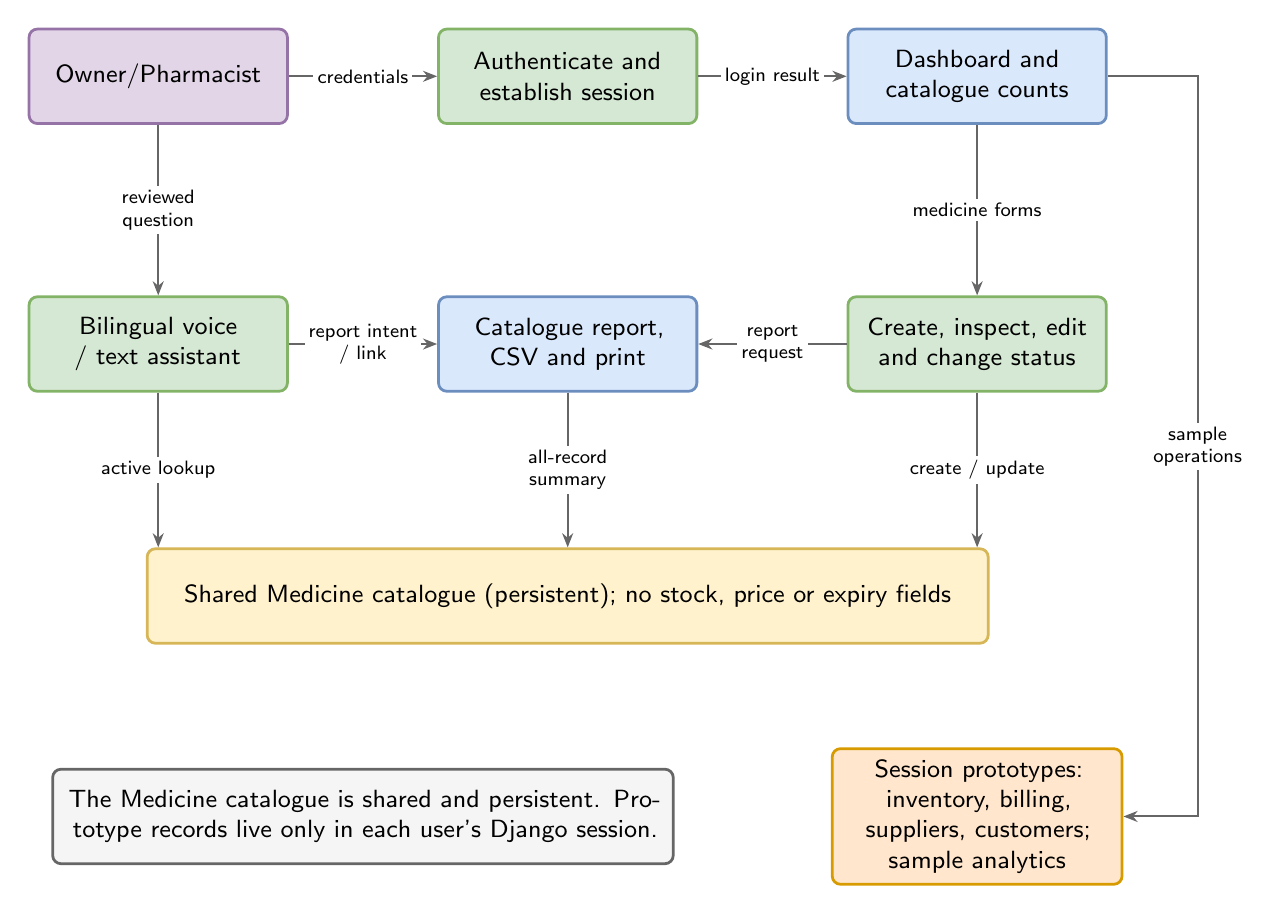
\begin{tikzpicture}
\node[actor,text width=30mm] (owner) at (0,0) {Owner/Pharmacist};
\node[process,text width=30mm] (auth) at (5.2,0) {Authenticate and establish session};
\node[ui,text width=30mm] (dash) at (10.4,0) {Dashboard and catalogue counts};
\node[process,text width=30mm] (voice) at (0,-3.4) {Bilingual voice / text assistant};
\node[ui,text width=30mm] (report) at (5.2,-3.4) {Catalogue report, CSV and print};
\node[process,text width=30mm] (cat) at (10.4,-3.4) {Create, inspect, edit and change status};
\node[store,text width=104mm] (db) at (5.2,-6.6) {Shared Medicine catalogue (persistent); no stock, price or expiry fields};
\node[prototype,text width=34mm] (demo) at (10.4,-9.4) {Session prototypes: inventory, billing, suppliers, customers; sample analytics};
\node[grey,text width=76mm] (nt) at (2.6,-9.4) {The Medicine catalogue is shared and persistent. Prototype records live only in each user's Django session.};
\draw[flow] (owner)--node[note]{credentials}(auth);
\draw[flow] (auth)--node[note]{login result}(dash);
\draw[flow] (dash)--node[note]{medicine forms}(cat);
\draw[flow] (owner)--node[note]{reviewed\\question}(voice);
\draw[flow] (cat)--node[note]{report\\request}(report);
\draw[flow] (voice)--node[note]{report intent\\/ link}(report);
\draw[flow] (voice.south)--node[note]{active lookup}(db.north -| voice.south);
\draw[flow] (report.south)--node[note]{all-record\\summary}(db.north -| report.south);
\draw[flow] (cat.south)--node[note]{create / update}(db.north -| cat.south);
\draw[flow] (dash.east)--(13.2,0)--node[note]{sample\\operations}(13.2,-9.4)--(demo.east);
\end{tikzpicture}
}
\caption{Current workflow. Authenticated catalogue functions use persistent medicine data; operational demo records remain session-scoped.}\label{fig:workflow}
\end{figure}

\subsection{Definitions, Acronyms and Abbreviations}\label{sec:terms}
\begin{longtable}{@{}L{32mm}L{124mm}@{}}
\caption{Definitions and abbreviations}\\
\toprule Term & Definition\\\midrule\endfirsthead
\toprule Term & Definition\\\midrule\endhead
\bottomrule\endfoot
SRS & Software Requirements Specification.\\
CSV & Comma-separated values, used for the catalogue export.\\
DFD & Data Flow Diagram: logical processes, data stores, external participants and exchanged information.\\
Catalogue & Master medicine descriptions and flags; it does not represent physical stock.\\
Session & Authenticated browser interaction identified by a session cookie, with server-side data in Django's configured session store.\\
Prototype record & Sample operational data serialized in a session, without its own shared business-domain table.\\
ORM & Object-relational mapper used by Django to access the configured relational database.\\
CSRF & Cross-Site Request Forgery; Django's CSRF token/middleware checks protect unsafe requests.\\
Voice assistant & Bounded, rule-based catalogue assistance with optional browser speech recognition and synthesis.\\
Acceptance criterion & A specific observation used to determine whether a stated requirement is satisfied under defined conditions.\\
RPO / RTO & Recovery point objective / recovery time objective; both remain to be agreed.\\
LLM & Large language model; no external LLM is used by this baseline.\\
API / HTTP & Application programming interface / Hypertext Transfer Protocol.\\
\end{longtable}

\subsection{References}\label{sec:references}
\begin{description}[style=nextline,leftmargin=12mm]
\item[R01] IEEE Std 830-1998, \emph{IEEE Recommended Practice for Software Requirements Specifications}. Historical structural reference, not a certification claim. \url{https://ieeexplore.ieee.org/document/720574}.
\item[R02] Django Software Foundation, \emph{Django documentation}. Consult documentation matching the recorded project version; this link does not change the baseline. \url{https://docs.djangoproject.com/}.
\item[R03] Python Software Foundation, \emph{Python 3.13 documentation}. \url{https://docs.python.org/3.13/}.
\item[R04] Supplied \emph{SAMS SRS v2.0}, used only for diagram appearance and structural ideas in this revision. None of its domain content is adopted.
\end{description}
Source identifiers below refer to the project working-tree files reviewed for this document. They identify evidence, not third-party product guarantees. File paths are relative to the project root; the supplied template is an external reference. The reference's project-specific statements are not authoritative for \Project.
\begin{description}[style=nextline,leftmargin=12mm]
\item[S01] \textbf{Reference SRS.} Supplied file \texttt{ryktphvctsxg.pdf}, ``Software Requirements Specification for IICT Website'', version 1.0, dated 24 August 2019, 11 pages. Used for chapter hierarchy and presentation only.
\item[S02] \textbf{Configuration and dependency baseline.} \Source{requirements.txt}; \Source{config/settings.py}; \Source{config/urls.py}; \Source{config/wsgi.py}; \Source{config/asgi.py}; \Source{manage.py}; \Source{.env.example}; \Source{.claude/launch.json}.
\item[S03] \textbf{Accounts.} \Source{apps/accounts/models.py}; \Source{apps/accounts/backends.py}; \Source{apps/accounts/forms.py}; \Source{apps/accounts/views.py}; \Source{apps/accounts/urls.py}; \Source{apps/accounts/admin.py}; initial account migration.
\item[S04] \textbf{Medicine domain.} \Source{apps/medicines/models.py}; \Source{apps/medicines/forms.py}; \Source{apps/medicines/views.py}; \Source{apps/medicines/urls.py}; \Source{apps/medicines/admin.py}; initial medicine migration.
\item[S05] \textbf{Dashboard and prototypes.} \Source{apps/core/views.py}; \Source{apps/core/urls.py}; \Source{templates/core/dashboard.html}; \Source{templates/core/module.html}; \Source{static/js/app.js}.
\item[S06] \textbf{Catalogue report.} \Source{apps/core/catalogue_report.py}; report view in \Source{apps/core/views.py}; \Source{templates/core/catalogue_report.html}; \Source{static/css/catalogue_report.css}; \Source{static/js/catalogue_report.js}.
\item[S07] \textbf{Assistant service and interface.} \Source{apps/core/assistant.py}; chat view in \Source{apps/core/views.py}; \Source{static/js/assistant.js}; \Source{templates/partials/_assistant.html}; \Source{docs/customer-assistant.md}.
\item[S08] \textbf{Shared presentation.} \Source{templates/base.html}; \Source{templates/base_app.html}; \Source{templates/partials/_sidebar.html}; account and medicine templates; \Source{static/css/tokens.css}; \Source{static/css/base.css}; \Source{static/css/app.css}; \Source{static/css/assistant.css}.
\item[S09] \textbf{Django verification sources.} \Source{apps/accounts/tests/test_login.py}; \Source{apps/medicines/tests/test_models.py}; \Source{apps/medicines/tests/test_views.py}; \Source{apps/core/tests.py}.
\item[S10] \textbf{Frontend verification source.} \Source{tests/assistant.test.cjs}. Speech event tests use simulation, not live microphone capture.
\end{description}


\clearpage
\section{Overall Description}
\subsection{Product Perspective}
\Project{} is a server-rendered web application implemented as a Django monolith. The browser renders Django templates and static HTML, CSS and JavaScript assets. Normal application forms use HTTP requests and server redirects. The voice assistant adds an asynchronous JSON request to the authenticated \texttt{/chat/} endpoint.

Three project applications are installed: \texttt{accounts}, \texttt{medicines} and \texttt{core}. Django supplies authentication, administration, sessions, messages, static-file handling and an object-relational mapper (ORM). There is no separate React client, REST framework, mobile application, message broker or external language-model service in the reviewed repository.

The default data store is SQLite. Setting PostgreSQL environment variables switches the configured database backend. Django's default database session backend also stores session records; consequently, the demo modules are \emph{session-scoped server data}, not relational inventory or billing tables and not merely browser local storage. Medicine records form one shared catalogue; the schema does not associate each medicine with a particular account or pharmacy tenant.

\subsection{User Classes and Characteristics}
The Owner/Pharmacist is one combined functional actor in this SRS and performs the pharmacy's authenticated operational activities. Supplier and Customer are additional business participants, represented by prototype contact records and assisted interactions; they do not have independent account types or portals in the current application. Django administration is a permission-controlled capability of an authorized account, not a separate business actor.
\begin{table}[H]
\centering\small
\caption{User classes and actual authorization boundaries}
\begin{tabularx}{\textwidth}{L{30mm}YY}
\toprule User class & Typical activities & Current access distinction\\\midrule
Owner/Pharmacist & Maintain catalogue, inspect dashboard, use reports and assistant, and manage prototype supplier/customer records. & Ordinary views require authentication. Access to \texttt{/admin/} additionally depends on Django staff status and permissions.\\
Supplier & Provide supplier contact information for pharmacy record keeping. & Represented by session-scoped prototype records maintained by the Owner/Pharmacist; no supplier login or portal.\\
Customer & Receive assistance with catalogue questions by text or voice at an authenticated counter session. & Contact records are session-scoped prototypes. No customer login or public assistant route is implemented.\\
Unauthenticated visitor & Open sign-in and password-help pages. & Protected pages redirect to login; the assistant endpoint returns an authentication error.\\
\bottomrule
\end{tabularx}
\end{table}

\begin{figure}[H]
\centering
\begin{lrbox}{\DiagramBox}\hyphenpenalty=10000 \exhyphenpenalty=10000 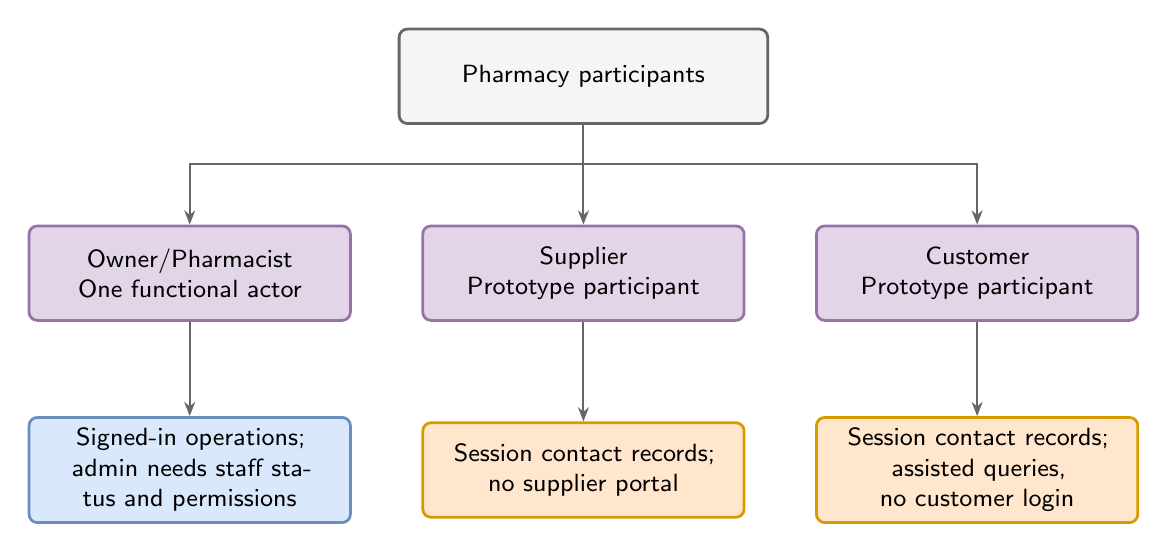
\begin{tikzpicture}
\node[grey,text width=44mm] (all) at (0,0) {Pharmacy participants};
\node[actor,text width=38mm] (owner) at (-5,-2.5) {Owner/Pharmacist\\One functional actor};
\node[actor,text width=38mm] (supplier) at (0,-2.5) {Supplier\\Prototype participant};
\node[actor,text width=38mm] (customer) at (5,-2.5) {Customer\\Prototype participant};
\node[ui,text width=38mm] (access) at (-5,-5) {Signed-in operations; admin needs staff status and permissions};
\node[prototype,text width=38mm] (contact) at (0,-5) {Session contact records; no supplier portal};
\node[prototype,text width=38mm] (assist) at (5,-5) {Session contact records; assisted queries, no customer login};
\draw[flow] (all.south)--++(0,-.5)-|(owner.north);
\draw[flow] (all)--(supplier);
\draw[flow] (all.south)--++(0,-.5)-|(customer.north);
\draw[flow] (owner)--(access);\draw[flow] (supplier)--(contact);\draw[flow] (customer)--(assist);
\end{tikzpicture}\end{lrbox}
\ifdim\wd\DiagramBox>\linewidth\resizebox{\linewidth}{!}{\usebox{\DiagramBox}}\else\usebox{\DiagramBox}\fi
\caption{User classification. Administration is a permission-controlled capability, not a separate pharmacy business actor.}\label{fig:users}
\end{figure}

\subsubsection{Users and Permissions}
\begin{table}[H]\centering\small
\caption{Users and permissions in the current baseline}\label{tab:permissions}
\begin{tabularx}{\textwidth}{@{}L{56mm}YYY@{}}
\toprule Resource / operation & Unauthenticated visitor & Owner/Pharmacist & Admin (staff / permissions)\\\midrule
Medicine application screens & No & C/R/U/A & C/R/U/A\\
Medicine deletion in application screens & No & No & No\\
Catalogue report / CSV & No & R & R\\
Voice/text assistant & No & Yes & Yes\\
Writable prototype modules & No & C/R/U/D & C/R/U/D\\
Analytics sample module & No & R & R\\
Django admin & No & No\textsuperscript{1} & Yes\textsuperscript{2}\\
Login with an active account & Yes & Yes & Yes\\
\bottomrule\end{tabularx}
\end{table}
\textbf{Matrix notes.} C = create, R = read, U = update, D = delete, A = activate/deactivate. Prototype C/R/U/D changes only session data. Application medicine operations use C/R/U/A, not deletion. Anonymous page requests redirect to login; anonymous chat returns 401 unless CSRF rejects it first. Login availability does not imply public registration.

\textsuperscript{1}The combined Owner/Pharmacist actor does not itself confer Django admin access. \textsuperscript{2}An active staff account may enter Django admin, but individual model operations depend on its assigned permissions; a superuser has framework-level privileges. Admin medicine deletion may be available with the appropriate permission and is not prohibited by the application-screen rule. Supplier/Customer participants have no independent login or portal. The stored \texttt{role} label is not an enforced authorization policy; NFR-SEC-06 remains Proposed.

\subsection{Product Functions}
\subsubsection{Implemented and prototype modules}
\begin{table}[H]
\centering\small
\caption{Module responsibilities and persistence}
\begin{tabularx}{\textwidth}{L{29mm}L{23mm}Y}
\toprule Module & Status & Responsibility and data source\\\midrule
Accounts & Implemented & Custom Django user, email/username authentication, login/logout and manual password-help guidance.\\
Medicines & Implemented & Database-backed catalogue with normalization, duplicate checks, filtering, details, editing and active/inactive status.\\
Dashboard & Implemented / mixed & Real medicine counts and recent additions alongside navigation and sample-module summaries.\\
Catalogue report & Implemented & All active and inactive medicines, category counts, prescription flags, CSV and print layout.\\
Voice assistant & Implemented & Deterministic catalogue queries and report intents; English/Hindi UI and replies; browser speech APIs.\\
Inventory & Prototype & Medicine label, quantity, reorder level, status and shelf fields stored as session sample records.\\
Billing & Prototype & Invoice, customer, item description, amount and status strings; no transaction calculation or stock deduction.\\
Suppliers / customers & Prototype & Session-scoped contact and status records; no foreign-key links to medicines, invoices or purchases.\\
Analytics & Prototype & Read-only sample metrics; no aggregation over operational transactions.\\
\bottomrule
\end{tabularx}
\end{table}

\subsubsection{System context and data flow}
The context diagram treats browser speech services as an external dependency. Their implementation and network use depend on the browser. The Django server receives the submitted text and selected language, not a microphone audio upload. The system does not automatically submit recognized speech; the user reviews the transcript and sends it explicitly.

\begin{figure}[H]
\centering
{\hyphenpenalty=10000 \exhyphenpenalty=10000
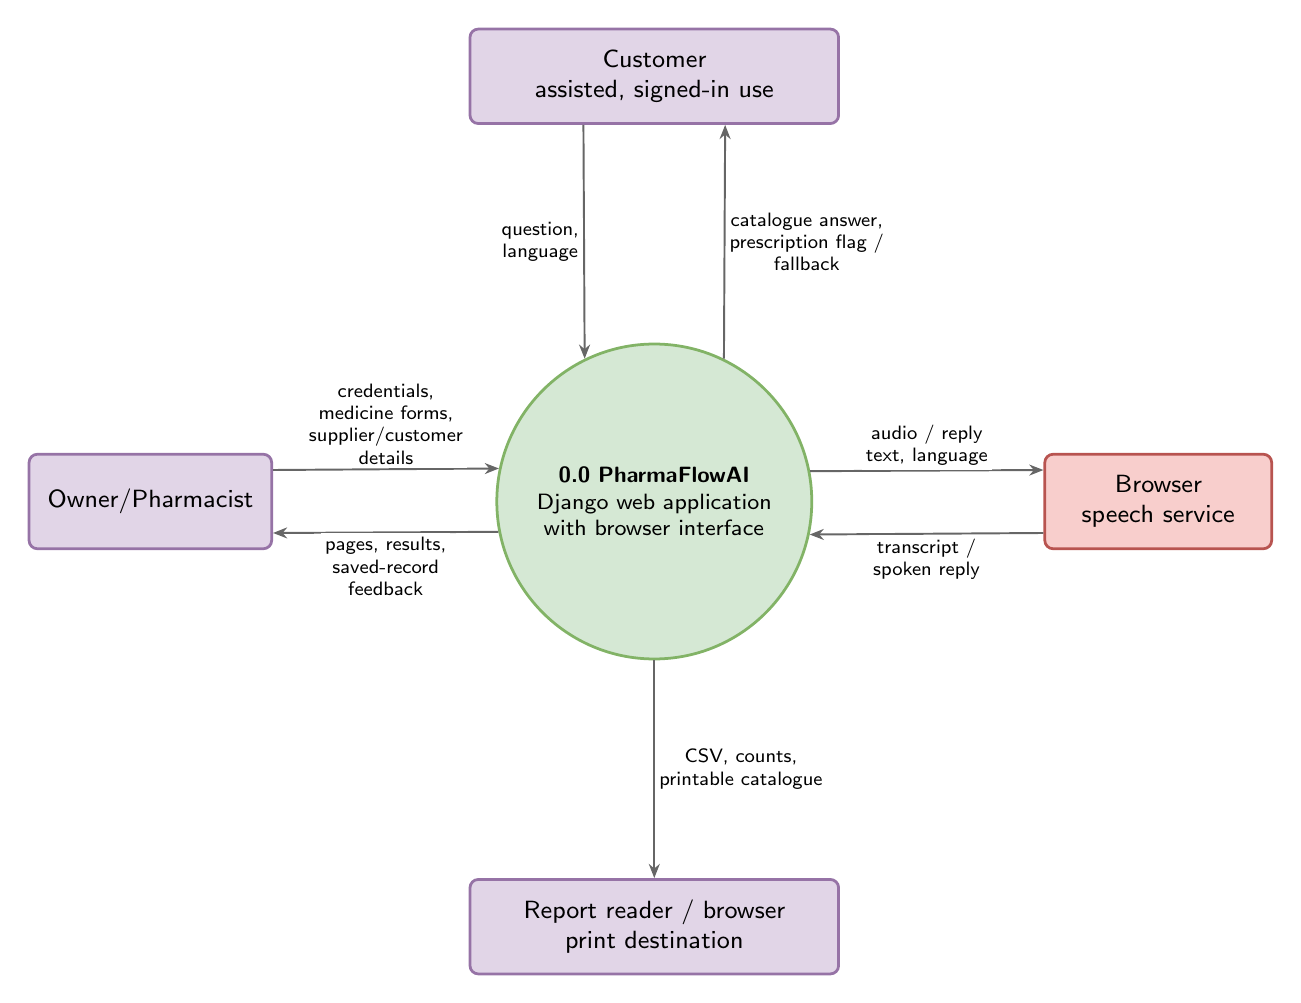
\begin{tikzpicture}
\node[dfdcircle,text width=30mm,minimum size=40mm] (sys) at (0,0) {\textbf{0.0 PharmaFlowAI}\\Django web application with browser interface};
\node[actor,text width=28mm] (staff) at (-6.4,0) {Owner/Pharmacist};
\node[boundary,text width=26mm] (speech) at (6.4,0) {Browser speech service};
\node[actor,text width=44mm] (cust) at (0,5.4) {Customer\\assisted, signed-in use};
\node[actor,text width=44mm] (reader) at (0,-5.4) {Report reader / browser print destination};
\draw[flow] ([yshift=4mm]staff.east)--node[above,note]{credentials,\\medicine forms,\\supplier/customer\\details}(sys.168.5);
\draw[flow] (sys.191.5)--node[below,note]{pages, results,\\saved-record\\feedback}([yshift=-4mm]staff.east);
\draw[flow] (sys.11.5)--node[above,note]{audio / reply\\text, language}([yshift=4mm]speech.west);
\draw[flow] ([yshift=-4mm]speech.west)--node[below,note]{transcript /\\spoken reply}(sys.348.5);
\draw[flow] ([xshift=-9mm]cust.south)--node[left,note]{question,\\language}(sys.116);
\draw[flow] (sys.64)--node[right,note]{catalogue answer,\\prescription flag /\\fallback}([xshift=9mm]cust.south);
\draw[flow] (sys.south)--node[right,note]{CSV, counts,\\printable catalogue}(reader.north);
\end{tikzpicture}
}
\caption{DFD Level 0. Customers use an authenticated counter session. Supplier details are entered by the Owner/Pharmacist; no supplier portal exists. Audio is processed through browser speech services, not uploaded to Django.}\label{fig:dfd0}
\end{figure}

\begin{figure}[H]
\centering
{\hyphenpenalty=10000 \exhyphenpenalty=10000
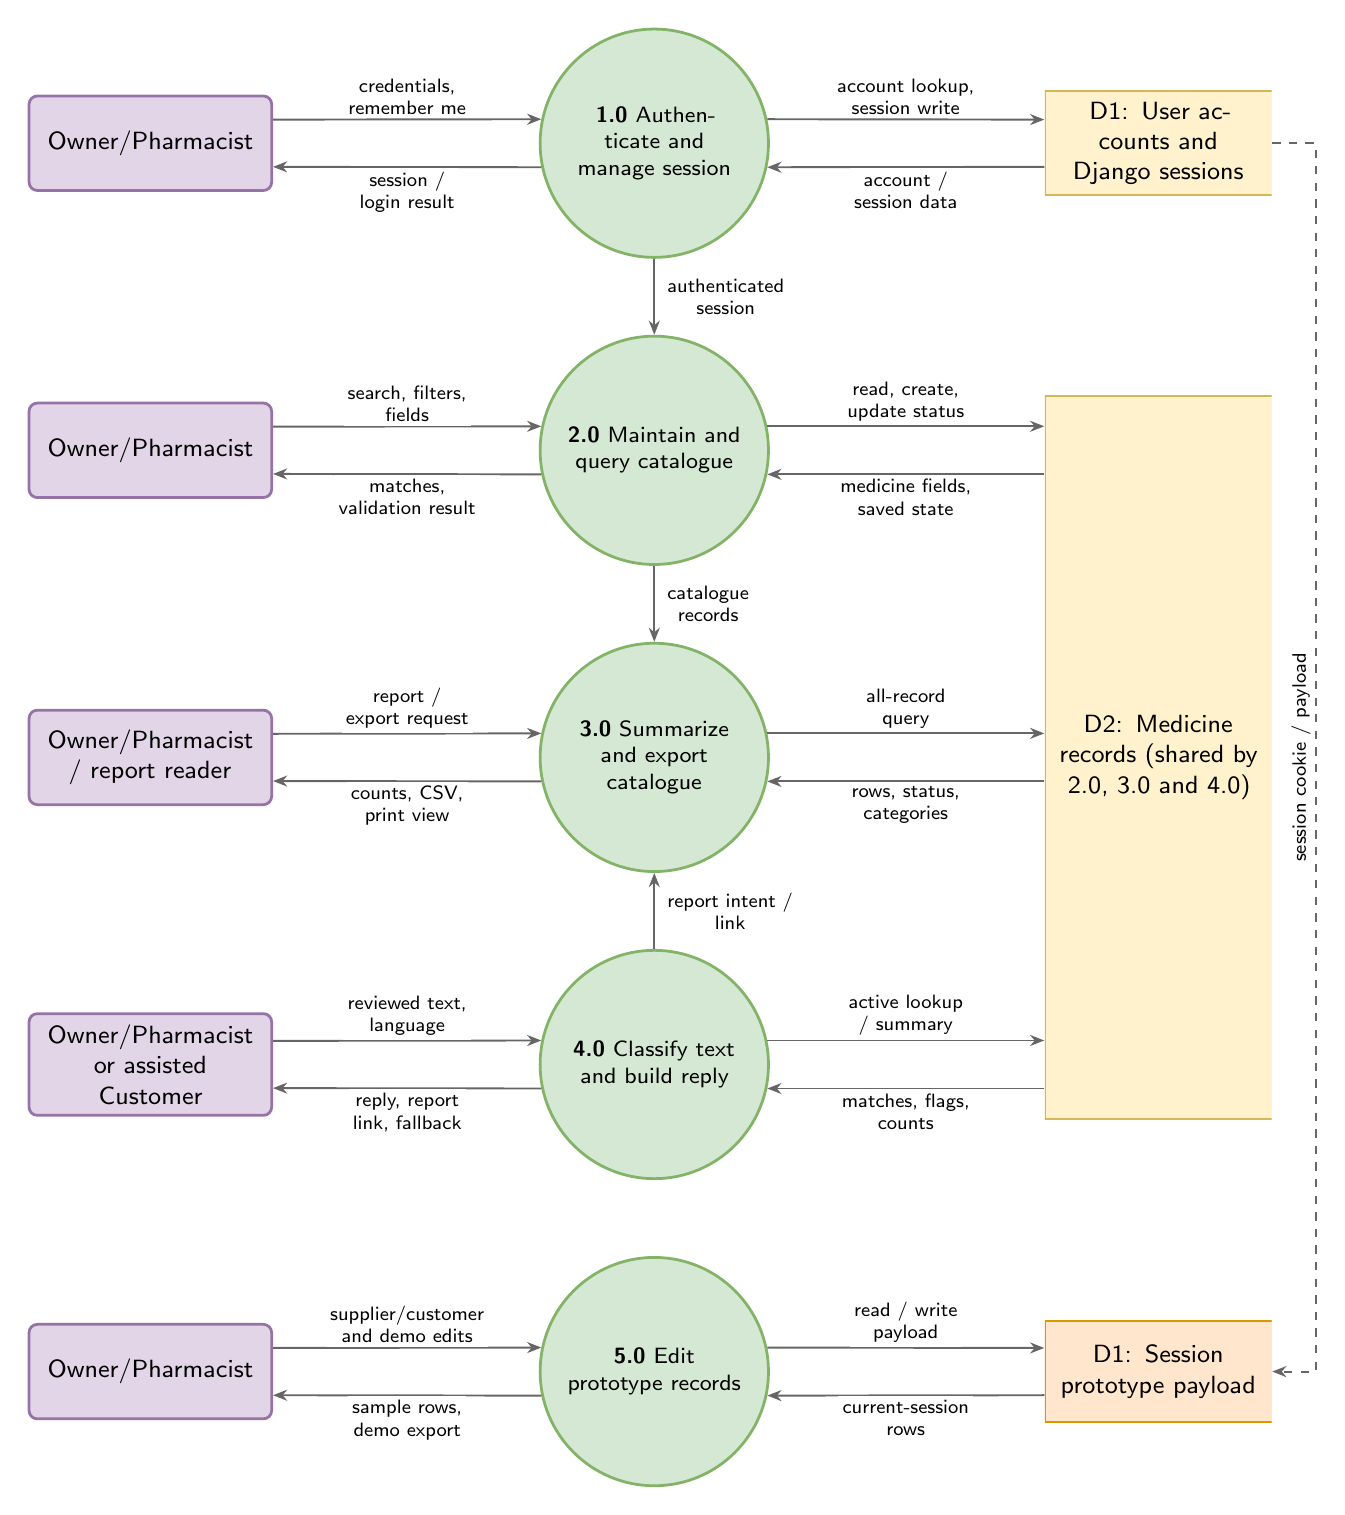
\begin{tikzpicture}
\node[dfdcircle,text width=22mm,minimum size=29mm] (p1) at (0,0) {\textbf{1.0} Authenticate and manage session};
\node[dfdcircle,text width=22mm,minimum size=29mm] (p2) at (0,-3.9) {\textbf{2.0} Maintain and query catalogue};
\node[dfdcircle,text width=22mm,minimum size=29mm] (p3) at (0,-7.8) {\textbf{3.0} Summarize and export catalogue};
\node[dfdcircle,text width=22mm,minimum size=29mm] (p4) at (0,-11.7) {\textbf{4.0} Classify text and build reply};
\node[dfdcircle,text width=22mm,minimum size=29mm] (p5) at (0,-15.6) {\textbf{5.0} Edit prototype records};
\node[actor,text width=28mm] (a1) at (-6.4,0) {Owner/Pharmacist};
\node[actor,text width=28mm] (a2) at (-6.4,-3.9) {Owner/Pharmacist};
\node[actor,text width=28mm] (a3) at (-6.4,-7.8) {Owner/Pharmacist\\/ report reader};
\node[actor,text width=28mm] (a4) at (-6.4,-11.7) {Owner/Pharmacist or assisted Customer};
\node[actor,text width=28mm] (a5) at (-6.4,-15.6) {Owner/Pharmacist};
\node[dfdstore,text width=26mm] (d1) at (6.4,0) {D1: User accounts and Django sessions};
\node[dfdstore,text width=26mm,minimum height=92mm] (d2) at (6.4,-7.8) {D2: Medicine records (shared by 2.0, 3.0 and 4.0)};
\node[dfdstore,fill=protoFill,text width=26mm,path picture={\draw[protoStroke,line width=1pt]
      (path picture bounding box.north east)--(path picture bounding box.north west)
      --(path picture bounding box.south west)--(path picture bounding box.south east);}] (d5) at (6.4,-15.6) {D1: Session prototype payload};
% actor <-> process flows
\foreach \i/\request/\response in {
1/{credentials,\\remember me}/{session /\\login result},
2/{search, filters,\\fields}/{matches,\\validation result},
3/{report /\\export request}/{counts, CSV,\\print view},
4/{reviewed text,\\language}/{reply, report\\link, fallback},
5/{supplier/customer\\and demo edits}/{sample rows,\\demo export}}{
  \draw[flow] ([yshift=3mm]a\i.east)--node[above,note]{\request}(p\i.168);
  \draw[flow] (p\i.192)--node[below,note]{\response}([yshift=-3mm]a\i.east);}
% process <-> data store flows
\draw[flow] (p1.12)--node[above,note]{account lookup,\\session write}([yshift=3mm]d1.west);
\draw[flow] ([yshift=-3mm]d1.west)--node[below,note]{account /\\session data}(p1.348);
\draw[flow] (p2.12)--node[above,note]{read, create,\\update status}(d2.west |- p2.12);
\draw[flow] (d2.west |- p2.348)--node[below,note]{medicine fields,\\saved state}(p2.348);
\draw[flow] (p3.12)--node[above,note]{all-record\\query}(d2.west |- p3.12);
\draw[flow] (d2.west |- p3.348)--node[below,note]{rows, status,\\categories}(p3.348);
\draw[flow] (p4.12)--node[above,note]{active lookup\\/ summary}(d2.west |- p4.12);
\draw[flow] (d2.west |- p4.348)--node[below,note]{matches, flags,\\counts}(p4.348);
\draw[flow] (p5.12)--node[above,note]{read / write\\payload}([yshift=3mm]d5.west);
\draw[flow] ([yshift=-3mm]d5.west)--node[below,note]{current-session\\rows}(p5.348);
% process <-> process flows
\draw[flow] (p1.south)--node[right,note,xshift=1mm]{authenticated\\session}(p2.north);
\draw[flow] (p2.south)--node[right,note,xshift=1mm]{catalogue\\records}(p3.north);
\draw[flow] (p4.north)--node[right,note,xshift=1mm]{report intent /\\link}(p3.south);
% shared session store linking 1.0 and 5.0
\draw[flow,dashed] (d1.east)--(8.4,0)--node[note,rotate=90,above]{session cookie / payload}(8.4,-15.6)--(d5.east);
\end{tikzpicture}
}
\caption{DFD Level 1. Repeated actors and D2 symbols denote the same participant or store. D1 contains framework sessions and the prototype payload, not an operational ledger. Processes 2.0--5.0 require an authenticated session; speech conversion surrounds process 4.0 in the browser.}\label{fig:dfd1}
\end{figure}

\subsubsection{Data model and data dictionary}
Two project-defined domain models are migrated: \texttt{accounts.User} and \texttt{medicines.Medicine}. Django adds framework tables for sessions, permissions, groups, content types and administration logs. No batch, invoice, customer or supplier domain models exist. No direct user-to-medicine foreign key exists.

\begin{table}[H]
\centering\small
\caption{Medicine entity data dictionary}
\begin{tabularx}{\textwidth}{L{46mm}L{28mm}Y}
\toprule Attribute & Type / size & Meaning and constraint\\\midrule
\texttt{id} & BigAutoField & Automatically generated primary key.\\
\texttt{name} & Char(200) & Required brand/product name; indexed.\\
\texttt{generic\_name} & Char(200) & Optional composition or generic name.\\
\texttt{strength} & Char(50) & Optional pack-strength text; not a dosage recommendation.\\
\texttt{category} & Char(100) & Optional free-text classification; indexed.\\
\texttt{manufacturer} & Char(150) & Optional manufacturer label.\\
\texttt{unit} & Char(20), choice & Tablet, capsule, syrup, injection, ointment, drops, sachet or other; default tablet.\\
\texttt{prescription\_required} & Boolean & Recorded prescription flag; default false. It is not legal or clinical verification.\\
\texttt{is\_active} & Boolean & Default true; inactive records remain readable.\\
\texttt{created\_at}, \texttt{updated\_at} & Date/time & Creation and latest-save timestamps.\\
\bottomrule
\end{tabularx}
\end{table}
Medicine text is normalized by trimming and collapsing whitespace. The combination of lowercased name, strength and manufacturer is unique at database level. The form provides a corresponding duplicate validation message. A composite index supports active-status/name access. There are no quantity, stock balance, expiry, cost or selling-price fields in this entity.

The custom User model extends Django's \texttt{AbstractUser}. It retains username, password hash, identity fields and framework permission attributes; email is unique and required by the model; \texttt{role} is a 20-character choice field defaulting to OWNER. Django's standard groups and permissions remain available. This legacy role metadata does not define separate business actors in this SRS: Owner/Pharmacist is one functional actor. Stored labels are not treated as an enforced authorization policy.

\begin{figure}[H]\centering
\begin{lrbox}{\DiagramBox}\hyphenpenalty=10000 \exhyphenpenalty=10000 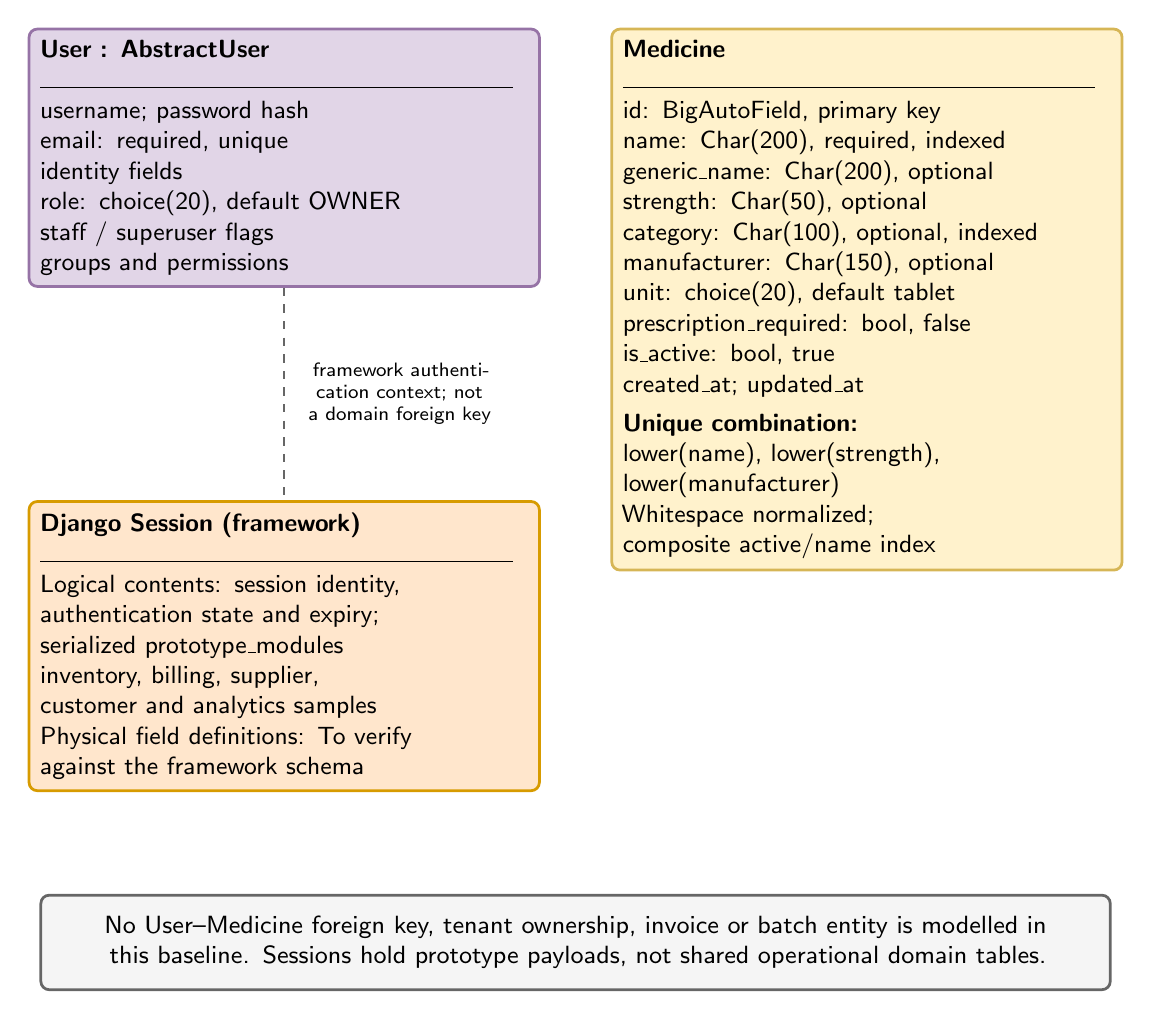
\begin{tikzpicture}
\node[classbox,fill=actorFill,draw=actorStroke,anchor=north] (user) at (-3.7,0) {
\textbf{User : AbstractUser}\\\rule{60mm}{.4pt}\\
username; password hash\\
email: required, unique\\
identity fields\\
role: choice(20), default OWNER\\
staff / superuser flags\\
groups and permissions};
\node[classbox,anchor=north] (medicine) at (3.7,0) {
\textbf{Medicine}\\\rule{60mm}{.4pt}\\
id: BigAutoField, primary key\\
name: Char(200), required, indexed\\
generic\_name: Char(200), optional\\
strength: Char(50), optional\\
category: Char(100), optional, indexed\\
manufacturer: Char(150), optional\\
unit: choice(20), default tablet\\
prescription\_required: bool, false\\
is\_active: bool, true\\
created\_at; updated\_at\\[3pt]
\textbf{Unique combination:}\\
lower(name), lower(strength),\\
lower(manufacturer)\\
Whitespace normalized;\\
composite active/name index};
\node[classbox,fill=protoFill,draw=protoStroke,anchor=north] (session) at (-3.7,-6) {
\textbf{Django Session (framework)}\\\rule{60mm}{.4pt}\\
Logical contents: session identity,\\
authentication state and expiry;\\
serialized prototype\_modules\\
inventory, billing, supplier,\\
customer and analytics samples\\
Physical field definitions: To verify\\
against the framework schema};
\draw[assoc,dashed] (user.south)--node[note,right,text width=28mm]{framework authentication context; not a domain foreign key}(session.north);
\node[grey,text width=133mm,anchor=north] at (0,-11) {No User--Medicine foreign key, tenant ownership, invoice or batch entity is modelled in this baseline. Sessions hold prototype payloads, not shared operational domain tables.};
\end{tikzpicture}\end{lrbox}
\ifdim\wd\DiagramBox>\linewidth\resizebox{\linewidth}{!}{\usebox{\DiagramBox}}\else\usebox{\DiagramBox}\fi
\caption{Class/ER view of the real domain and framework session store. Session attributes are shown conceptually because the source SRS does not enumerate its physical schema.}\label{fig:er}
\end{figure}

\subsection{Operating Environment}
\begin{table}[H]
\centering\small
\caption{Verified technology baseline and conditional dependencies}
\begin{tabularx}{\textwidth}{L{37mm}Y}
\toprule Component & Baseline\\\midrule
Runtime / framework & Python 3.13.9 and Django 6.1 observed in the local environment; the development launcher selects Python 3.13.\\
Declared dependencies & Django 6.1, python-dotenv 1.1.1 and psycopg[binary] 3.2.10 in \texttt{requirements.txt}. Dependency installation on every platform is not verified.\\
Frontend & Django templates, HTML, CSS design tokens and plain JavaScript. Node.js runs assistant unit tests; it is not the application's web backend.\\
Database & SQLite by default; PostgreSQL backend selected when \texttt{POSTGRES\_DB} is supplied. No production database deployment is assumed.\\
Web serving & Local Django development server; WSGI and ASGI entry points exist. Production server and hosting provider are unspecified.\\
Speech & Browser \texttt{SpeechRecognition}/\texttt{webkitSpeechRecognition} and \texttt{speechSynthesis}; availability and voices vary by device.\\
Client / hardware & A supported browser and display/keyboard for text use. Microphone and permission for voice input; speaker/headphones for audio output. No measured minimum CPU/RAM specification is established.\\
Network / configuration & Localhost for development or HTTPS for deployed microphone use. Browser speech services may require internet. Optional \texttt{.env} configuration; default time zone Asia/Kolkata.\\
\bottomrule
\end{tabularx}
\end{table}
Windows is the evidenced development environment. Other platforms may run the underlying technologies, but cross-platform acceptance testing is not evidenced. Speech input is an optional enhancement: unsupported browsers must retain text interaction. Security settings available outside debug mode include HTTPS redirection, secure cookies and HSTS; their correct deployment depends on configuration and a trusted reverse-proxy arrangement.

\subsection{Design}
\subsubsection{Architecture and deployment boundary}
\begin{figure}[H]
\centering
\begin{lrbox}{\DiagramBox}\hyphenpenalty=10000 \exhyphenpenalty=10000 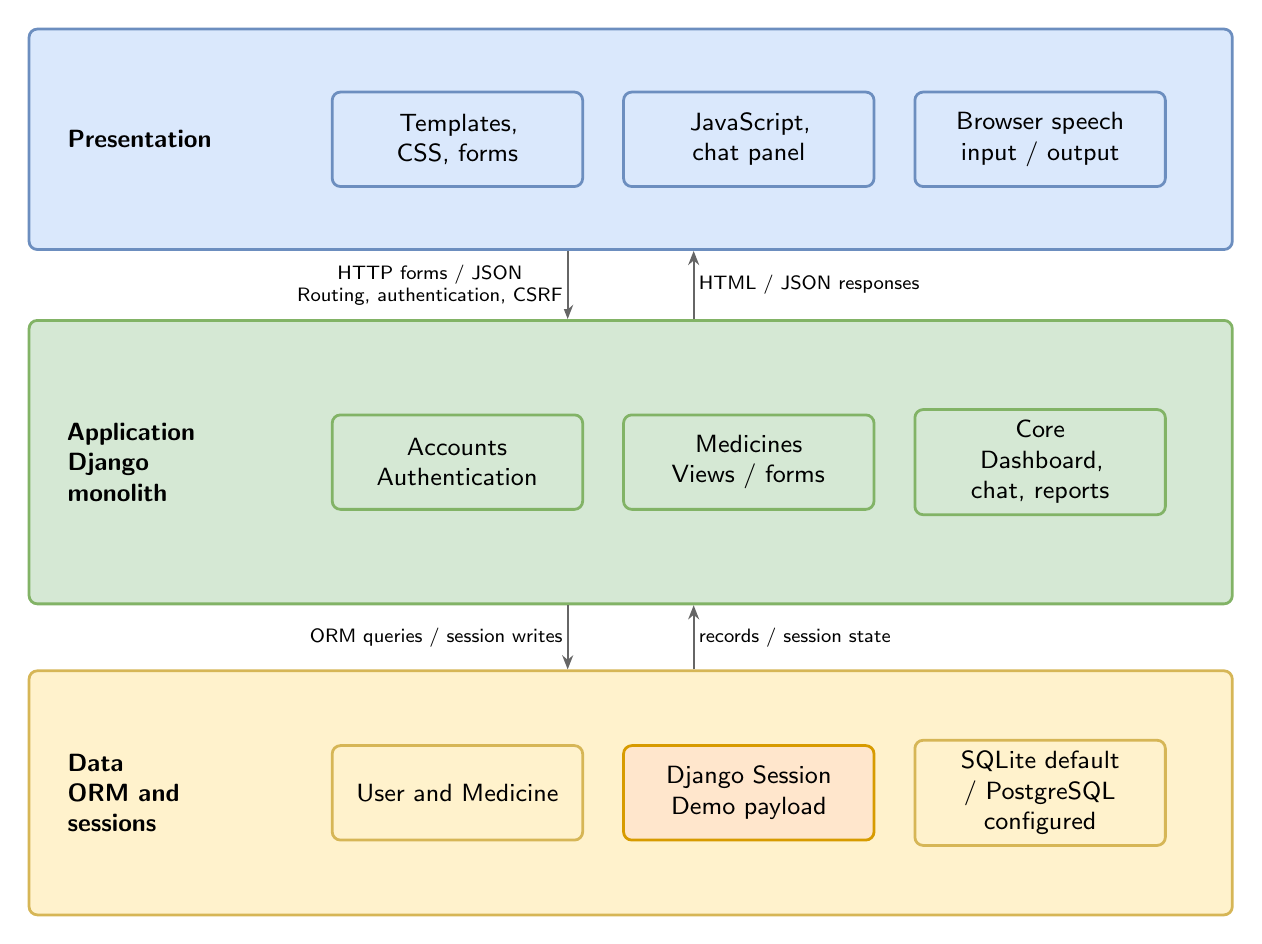
\begin{tikzpicture}
\node[band,minimum height=28mm] (ui) at (0,0) {};
\node[font=\sffamily\small\bfseries,align=left,text width=25mm] at (-5.9,0) {Presentation};
\node[ui,text width=29mm] at (-2.2,0) {Templates, CSS, forms};
\node[ui,text width=29mm] at (1.5,0) {JavaScript, chat panel};
\node[ui,text width=29mm] at (5.2,0) {Browser speech input / output};
\node[band,fill=logicFill,draw=logicStroke,minimum height=36mm] (logic) at (0,-4.1) {};
\node[font=\sffamily\small\bfseries,align=left,text width=24mm] at (-5.95,-4.1) {Application\\Django\\monolith};
\node[process,text width=29mm] at (-2.2,-4.1) {Accounts\\Authentication};
\node[process,text width=29mm] at (1.5,-4.1) {Medicines\\Views / forms};
\node[process,text width=29mm] at (5.2,-4.1) {Core\\Dashboard, chat, reports};
\node[band,fill=dataFill,draw=dataStroke,minimum height=31mm] (data) at (0,-8.3) {};
\node[font=\sffamily\small\bfseries,align=left,text width=25mm] at (-5.9,-8.3) {Data\\ORM and\\sessions};
\node[store,text width=29mm] at (-2.2,-8.3) {User and Medicine};
\node[prototype,text width=29mm] at (1.5,-8.3) {Django Session\\Demo payload};
\node[store,text width=29mm] at (5.2,-8.3) {SQLite default / PostgreSQL configured};
\draw[flow] ([xshift=-8mm]ui.south)--node[note,left]{HTTP forms / JSON\\Routing, authentication, CSRF}([xshift=-8mm]logic.north);
\draw[flow] ([xshift=8mm]logic.north)--node[note,right]{HTML / JSON responses}([xshift=8mm]ui.south);
\draw[flow] ([xshift=-8mm]logic.south)--node[note,left]{ORM queries / session writes}([xshift=-8mm]data.north);
\draw[flow] ([xshift=8mm]data.north)--node[note,right]{records / session state}([xshift=8mm]logic.south);
\end{tikzpicture}\end{lrbox}
\ifdim\wd\DiagramBox>\linewidth\resizebox{\linewidth}{!}{\usebox{\DiagramBox}}\else\usebox{\DiagramBox}\fi
\caption{Layered component architecture. All application modules share the Django monolith. WSGI/ASGI hooks and PostgreSQL configuration do not establish production deployment.}\label{fig:architecture}
\end{figure}

\subsubsection{Design and Implementation Constraints}
\begin{itemize}
\item \textbf{Framework/runtime:} retain the recorded Django monolith and Python 3.13 development family; the observed versions are Django 6.1 and Python 3.13.9. No additional API framework or frontend application is assumed.
\item \textbf{Persistence:} SQLite is the default; PostgreSQL is configurable but its production deployment is not established. Operational demos stay session-scoped until a separate domain-model change is accepted.
\item \textbf{Assistant:} classification uses explicit rules, aliases and catalogue queries, with no external LLM. Browser speech availability, language voices, permission and possible online processing constrain voice use.
\item \textbf{Development evidence:} Windows is the evidenced host; other platforms and minimum hardware specifications are To verify.
\item \textbf{Academic timeline:} delivery must fit the course schedule, but deadlines and milestones are To verify and are not invented here.
\item \textbf{Tools/cost:} free/open-source development tools are the requested planning constraint; a complete dependency/licence inventory and any hosting or speech-provider charges are To verify. No zero-cost deployment claim is made.
\end{itemize}

\subsubsection{External interfaces}
The primary user interface consists of sign-in, dashboard, medicine list/detail/form, prototype module, catalogue report and voice-assistant panel screens. Forms include CSRF tokens. JavaScript progressively enhances navigation, table search/export, password visibility and the assistant. The assistant requires JavaScript; ordinary server-rendered catalogue operations are not a single-page application.

\begin{table}[H]
\centering\small
\caption{Principal HTTP interfaces}
\begin{tabularx}{\textwidth}{L{53mm}L{24mm}Y}
\toprule Route & Methods & Purpose / access\\\midrule
\texttt{/accounts/login/} & GET, POST & Display sign-in and authenticate.\\
\texttt{/accounts/logout/} & POST & End the session; GET is disallowed.\\
\texttt{/accounts/password-help/} & GET & Explain manual reset through administration.\\
\texttt{/dashboard/} & GET & Authenticated dashboard.\\
\texttt{/medicines/} & GET & Authenticated search/filter/sort list.\\
\texttt{/medicines/add/},\newline\texttt{/medicines/<id>/edit/} & GET, POST & Authenticated creation / editing.\\
\texttt{/medicines/<id>/},\newline\texttt{/medicines/<id>/status/} & GET; POST & Inspect record; change status respectively.\\
\texttt{/modules/<slug>/} & GET & Authenticated prototype view. Separate \texttt{save/} and \texttt{delete/} routes accept POST.\\
\texttt{/reports/medicine-catalogue/} & GET & Authenticated full report; \texttt{?format=csv} exports CSV.\\
\texttt{/chat/} & POST & Authenticated JSON assistant; CSRF required.\\
\texttt{/admin/} & Framework routes & Django administration; staff status and permissions apply.\\
\bottomrule
\end{tabularx}
\end{table}

The assistant request object contains a string \texttt{message} and optional \texttt{language}, which defaults to \texttt{en-IN}; \texttt{hi-IN} is the other allowed value. After trimming, messages must contain 1--500 characters. The view rejects request bodies larger than 8,192 bytes. Successful responses contain \texttt{reply}, \texttt{medicines} and, for report intents, \texttt{report\_url}. Each medicine result contains name, generic name and prescription flag. The frontend accepts a report link only when it equals the server-rendered, same-application report path.

Validation errors use HTTP 400; the assistant view uses 401 when authentication is missing; CSRF rejection uses 403; oversized bodies checked by the view use 413. Django may reject requests earlier through its own request-size handling. Report and successful chat responses specify \texttt{Cache-Control: no-store}. Browser printing can save a PDF where supported; no server-side PDF generation service is implemented.

\subsubsection{Catalogue activity}
\begin{figure}[H]
\centering
\begin{lrbox}{\DiagramBox}\hyphenpenalty=10000 \exhyphenpenalty=10000 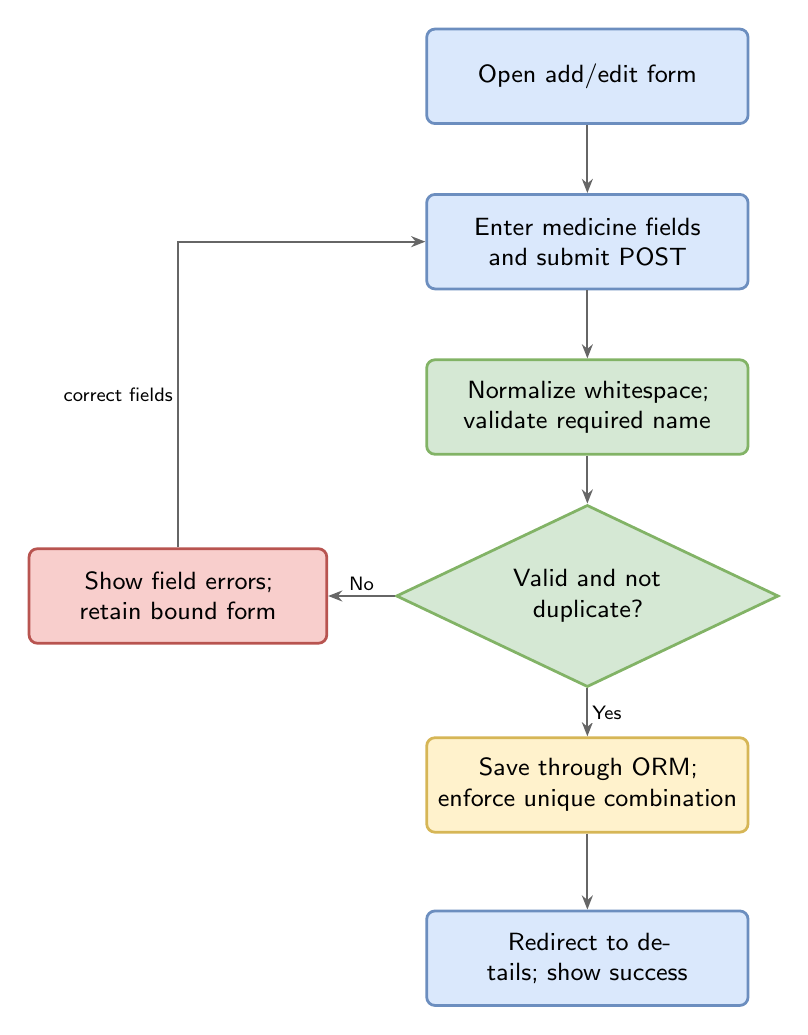
\begin{tikzpicture}
\node[ui,text width=38mm] (open) at (0,0) {Open add/edit form};
\node[ui,text width=38mm] (submit) at (0,-2.1) {Enter medicine fields and submit POST};
\node[process,text width=38mm] (norm) at (0,-4.2) {Normalize whitespace; validate required name};
\node[decision,text width=28mm] (valid) at (0,-6.6) {Valid and not duplicate?};
\node[boundary,text width=35mm] (error) at (-5.2,-6.6) {Show field errors; retain bound form};
\node[store,text width=38mm] (save) at (0,-9) {Save through ORM; enforce unique combination};
\node[ui,text width=38mm] (detail) at (0,-11.2) {Redirect to details; show success};
\draw[flow] (open)--(submit);\draw[flow] (submit)--(norm);\draw[flow] (norm)--(valid);
\draw[flow] (valid)--node[note,above]{No}(error);
\draw[flow] (error.north)|-node[note,pos=.25,left]{correct fields}(submit.west);
\draw[flow] (valid)--node[note,right]{Yes}(save);\draw[flow] (save)--(detail);
\end{tikzpicture}\end{lrbox}
\ifdim\wd\DiagramBox>\linewidth\resizebox{\linewidth}{!}{\usebox{\DiagramBox}}\else\usebox{\DiagramBox}\fi
\caption{Catalogue creation/edit activity. Invalid submissions retain the form. Separate POST status actions deactivate or reactivate records; application forms do not delete medicines.}\label{fig:activity}
\end{figure}

\subsubsection{Voice-assistant interaction}
\begin{figure}[H]
\centering
{\hyphenpenalty=10000 \exhyphenpenalty=10000
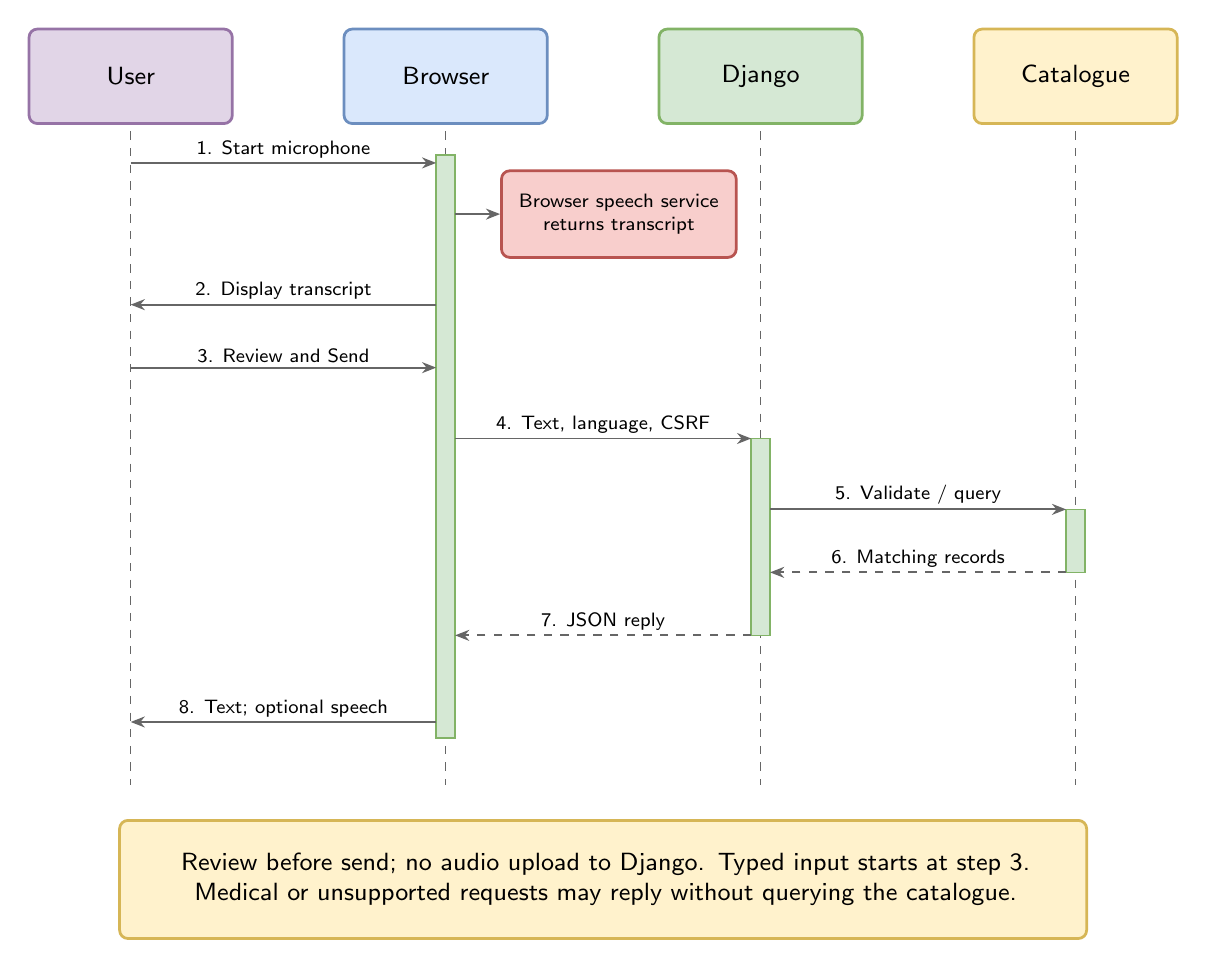
\begin{tikzpicture}
\node[actor,text width=23mm] at (0,0) {User};
\node[ui,text width=23mm] at (4,0) {Browser};
\node[process,text width=23mm] at (8,0) {Django};
\node[store,text width=23mm] at (12,0) {Catalogue};
\foreach \x in {0,4,8,12}{\draw[life] (\x,-.7)--(\x,-9);}
\draw[activation] (3.88,-1) rectangle (4.12,-8.4);
\draw[activation] (7.88,-4.6) rectangle (8.12,-7.1);
\draw[activation] (11.88,-5.5) rectangle (12.12,-6.3);
\draw[flow] (0,-1.1)--node[note,above]{1. Start microphone}(3.88,-1.1);
\node[boundary,text width=27mm,minimum height=11mm,font=\sffamily\scriptsize] (speech) at (6.2,-1.75) {Browser speech service returns transcript};
\draw[flow] (4.12,-1.75)--(speech.west);
\draw[flow] (3.88,-2.9)--node[note,above]{2. Display transcript}(0,-2.9);
\draw[flow] (0,-3.7)--node[note,above]{3. Review and Send}(3.88,-3.7);
\draw[flow] (4.12,-4.6)--node[note,above]{4. Text, language, CSRF}(7.88,-4.6);
\draw[flow] (8.12,-5.5)--node[note,above]{5. Validate / query}(11.88,-5.5);
\draw[flow,dashed] (11.88,-6.3)--node[note,above]{6. Matching records}(8.12,-6.3);
\draw[flow,dashed] (7.88,-7.1)--node[note,above]{7. JSON reply}(4.12,-7.1);
\draw[flow] (3.88,-8.2)--node[note,above]{8. Text; optional speech}(0,-8.2);
\node[store,text width=120mm,minimum height=15mm] at (6,-10.2) {Review before send; no audio upload to Django. Typed input starts at step 3. Medical or unsupported requests may reply without querying the catalogue.};
\end{tikzpicture}
}
\caption{Voice-assistant sequence with activation bars. Recognition and speech synthesis are browser-dependent; Django receives reviewed text and language only.}\label{fig:voice-sequence}
\end{figure}
The backend classifies text using explicit patterns, aliases and token matching. It does not retain conversation context or call a language model. A single lookup returns up to five active medicine results, while report requests summarize all active and inactive catalogue entries. Medical-pattern handling is a bounded rule set rather than a validated clinical classifier. Speech is single-turn, with review before transmission and optional playback afterward.

\subsubsection{State behaviour}
\begin{figure}[H]\centering
\begin{lrbox}{\DiagramBox}\hyphenpenalty=10000 \exhyphenpenalty=10000 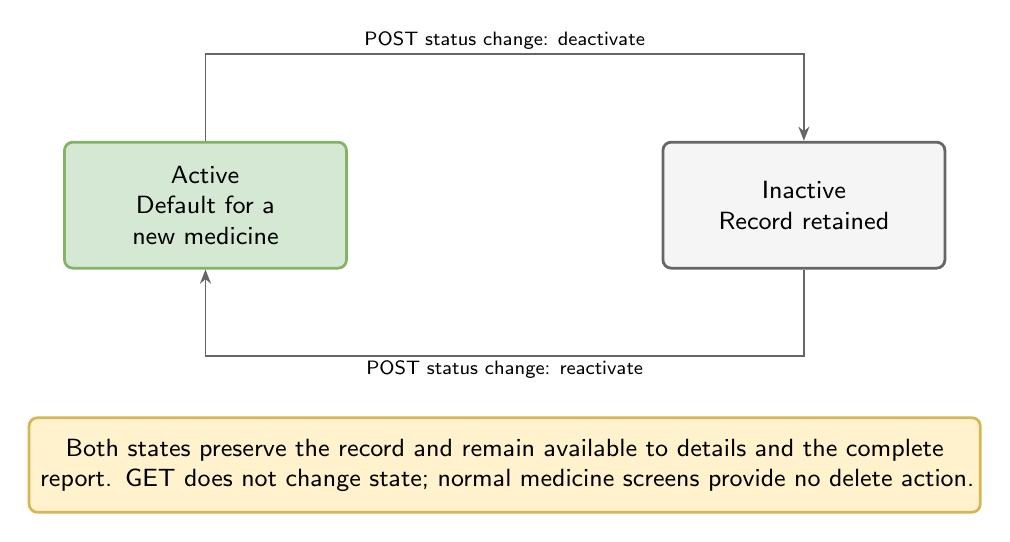
\begin{tikzpicture}
\node[process,text width=33mm,minimum height=16mm] (active) at (-3.8,0) {Active\\Default for a new medicine};
\node[grey,text width=33mm,minimum height=16mm] (inactive) at (3.8,0) {Inactive\\Record retained};
\draw[flow] (active.north)--++(0,1.1)-|node[note,pos=.25,above]{POST status change: deactivate}(inactive.north);
\draw[flow] (inactive.south)--++(0,-1.1)-|node[note,pos=.25,below]{POST status change: reactivate}(active.south);
\node[store,text width=118mm] at (0,-3.3) {Both states preserve the record and remain available to details and the complete report. GET does not change state; normal medicine screens provide no delete action.};
\end{tikzpicture}\end{lrbox}
\ifdim\wd\DiagramBox>\linewidth\resizebox{\linewidth}{!}{\usebox{\DiagramBox}}\else\usebox{\DiagramBox}\fi
\caption{Medicine state diagram. POST status actions update the flag and timestamp without deleting the record.}\label{fig:medicine-state}
\end{figure}
\begin{figure}[H]
\centering
{\hyphenpenalty=10000 \exhyphenpenalty=10000
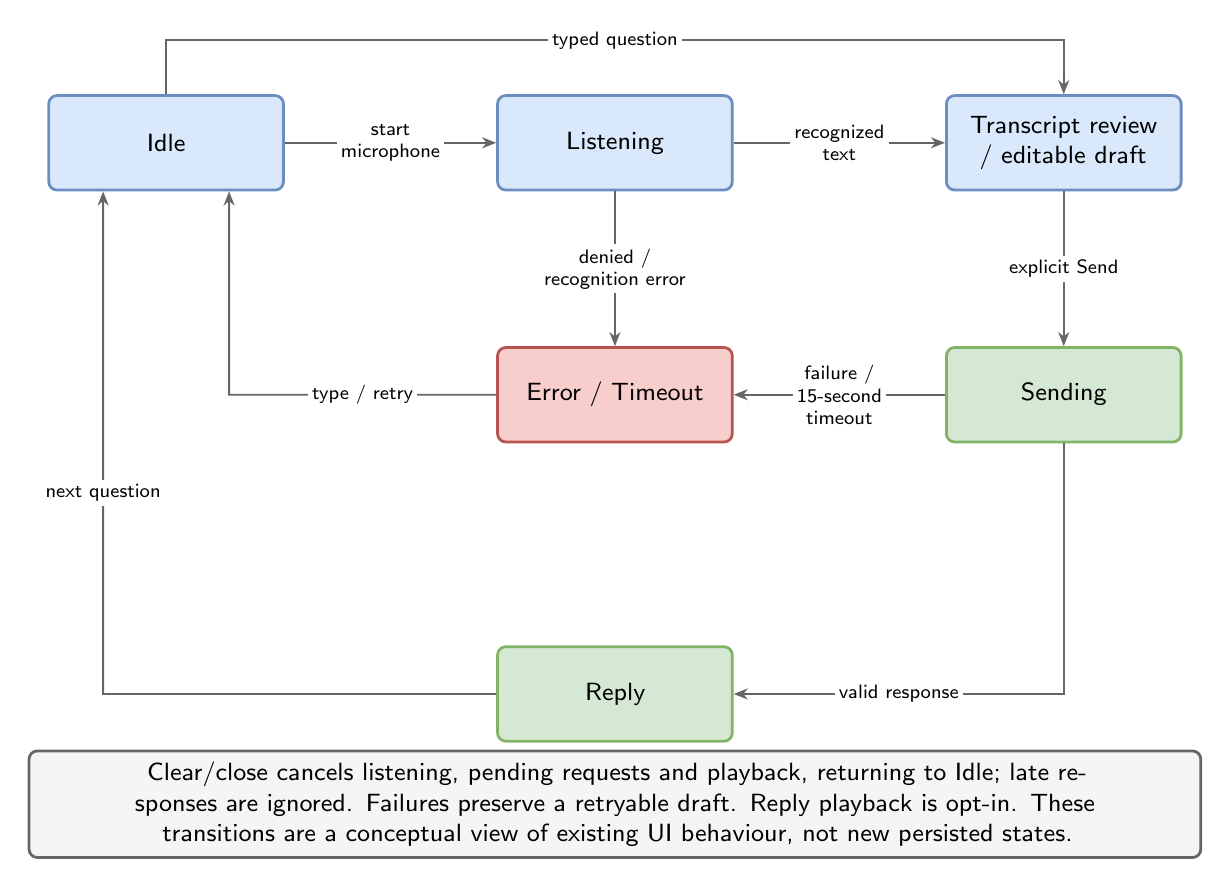
\begin{tikzpicture}
\node[ui,text width=27mm] (idle) at (0,0) {Idle};
\node[ui,text width=27mm] (listen) at (5.7,0) {Listening};
\node[ui,text width=27mm] (review) at (11.4,0) {Transcript review / editable draft};
\node[boundary,text width=27mm] (err) at (5.7,-3.2) {Error / Timeout};
\node[process,text width=27mm] (send) at (11.4,-3.2) {Sending};
\node[process,text width=27mm] (reply) at (5.7,-7.0) {Reply};
\draw[flow] (idle)--node[note]{start\\microphone}(listen);
\draw[flow] (listen)--node[note]{recognized\\text}(review);
\draw[flow] (idle.north)--(0,1.3)--node[note]{typed question}(11.4,1.3)--(review.north);
\draw[flow] (review)--node[note]{explicit Send}(send);
\draw[flow] (listen)--node[note]{denied /\\recognition error}(err);
\draw[flow] (send)--node[note]{failure /\\15-second\\timeout}(err);
\draw[flow] (send.south)--(11.4,-7.0)--node[note]{valid response}(reply.east);
\draw[flow] (err.west)--node[note]{type / retry}(0.8,-3.2)--([xshift=8mm]idle.south);
\draw[flow] (reply.west)--(-0.8,-7.0)--node[note,pos=.4]{next question}([xshift=-8mm]idle.south);
\node[grey,text width=146mm] at (5.7,-8.4) {Clear/close cancels listening, pending requests and playback, returning to Idle; late responses are ignored. Failures preserve a retryable draft. Reply playback is opt-in. These transitions are a conceptual view of existing UI behaviour, not new persisted states.};
\end{tikzpicture}
}
\caption{Assistant request states. Typed input bypasses Listening; recognition never sends automatically.}\label{fig:assistant-state}
\end{figure}

\clearpage
\section{System Features}
\subsection{Description and Priority}
Features are prioritized according to their role in a usable catalogue application. High priority denotes core access, data integrity and supported outputs; medium priority denotes convenience or demonstration functions. Prototype priority does not imply readiness for real transactions.
\begin{table}[H]
\centering\small
\caption{Feature priorities}
\begin{tabularx}{\textwidth}{L{35mm}L{19mm}L{24mm}Y}
\toprule Feature & Priority & State & Rationale\\\midrule
Authentication & High & Implemented & Establish access to shared pharmacy data and end sessions correctly.\\
Medicine maintenance & High & Implemented & Maintain the master data used by catalogue views and reports.\\
Search and dashboard & High & Implemented & Locate records and inspect actual catalogue counts.\\
Catalogue report & High & Implemented & Provide a complete, exportable register with clear data limitations.\\
Voice/text assistant & Medium & Implemented & Offer bilingual catalogue access without promising live stock or medical advice.\\
Operational modules & Medium & Prototype & Demonstrate proposed workflows for later domain-model development.\\
Transactional inventory / billing & Medium & Proposed & Requires models, integrity rules and business decisions absent from the current system.\\
\bottomrule
\end{tabularx}
\end{table}

\subsection{Functional Requirements}
The acceptance criteria below define concrete checks against the reviewed baseline. They are not a statement that every manual scenario, environment or concurrency condition has already passed. The verification mapping in Section 5.3 distinguishes automated evidence from remaining validation.

\subsubsection{Accounts and authentication}
All requirements in Table~\ref{tab:auth} are implemented and high priority, except password-help guidance, which is medium priority. Sources: S02, S03 and S09 in Section~\ref{sec:references}.
\begingroup\small\setlength{\tabcolsep}{4pt}
\begin{longtable}{@{}L{25mm}L{88mm}L{16mm}L{22mm}@{}}
\caption{Authentication requirements and acceptance criteria}\label{tab:auth}\\
\toprule ID & Requirement & Priority & Status\\\midrule\endfirsthead
\toprule ID & Requirement & Priority & Status\\\midrule\endhead
\bottomrule\endfoot
FR-AUTH-01 & The system shall authenticate an active account using a username or email and a valid password. & High & Implemented\\*
\Criterion{Valid credentials reach the dashboard or an accepted local next-page URL. An email lookup is case-insensitive.}
FR-AUTH-02 & The system shall reject incorrect credentials and inactive accounts without authenticating them. & High & Implemented\\*
\Criterion{Incorrect or unknown credentials produce a generic failure message; an inactive user does not acquire an authenticated session.}
FR-AUTH-03 & The system shall apply the selected Remember me session policy. & High & Implemented\\*
\Criterion{Checked: session expiry uses the configured age, default 14 days. Unchecked: expiry is set to browser-close semantics. Browser restoration behaviour is outside the application guarantee.}
FR-AUTH-04 & The system shall protect dashboard, medicine, module and report access through login requirements. & High & Implemented\\*
\Criterion{Anonymous requests redirect to login. Anonymous chat POST requests return HTTP 401 when not rejected earlier by CSRF middleware.}
FR-AUTH-05 & The system shall accept sign-out through POST and flush the authenticated session. & High & Implemented\\*
\Criterion{GET logout is rejected; POST logout returns to sign-in with confirmation and subsequent protected access requires login.}
FR-AUTH-06 & The system shall restrict post-login and post-status-change redirects to accepted local destinations. & High & Implemented\\*
\Criterion{A normal local next URL is honoured; an external next URL is ignored in favour of the default destination.}
FR-AUTH-07 & The password-help page shall explain the manual administrator reset path. & Medium & Implemented\\*
\Criterion{The page states that self-service email recovery is unavailable; it does not claim to send a reset email.}
\end{longtable}
\endgroup

\subsubsection{Medicine catalogue and dashboard}
All requirements in Table~\ref{tab:medicine} are implemented and high priority. Sources: S04, S05, S06 and S09.
\begingroup\small\setlength{\tabcolsep}{4pt}
\begin{longtable}{@{}L{25mm}L{88mm}L{16mm}L{22mm}@{}}
\caption{Catalogue and dashboard requirements}\label{tab:medicine}\\
\toprule ID & Requirement & Priority & Status\\\midrule\endfirsthead
\toprule ID & Requirement & Priority & Status\\\midrule\endhead
\bottomrule\endfoot
FR-MED-01 & The system shall create a medicine with its supported master-data fields and require a non-blank name. & High & Implemented\\*
\Criterion{A valid submission creates a database record and redirects to details. A missing or whitespace-only name displays validation errors.}
FR-MED-02 & The system shall normalize medicine text and reject duplicate name/strength/manufacturer combinations case-insensitively. & High & Implemented\\*
\Criterion{Extra internal and edge whitespace is normalized; an equivalent duplicate fails validation. Different strength or manufacturer is allowed.}
FR-MED-03 & The system shall permit inspection and editing of an existing medicine. & High & Implemented\\*
\Criterion{Details show stored data; the edit form is prefilled; a valid edit persists. A nonexistent identifier returns HTTP 404.}
FR-MED-04 & The application shall toggle active/inactive status through POST without deleting the medicine. & High & Implemented\\*
\Criterion{POST changes the flag, updates the timestamp and shows confirmation. GET does not mutate state; reactivation is possible.}
FR-MED-05 & The list shall search medicine name, generic name and manufacturer and filter by status and category. & High & Implemented\\*
\Criterion{A matching query narrows results; default status is active. Invalid form filters fall back to the defined defaults.}
FR-MED-06 & The list shall support the defined sort options and paginate at 20 records per page. & High & Implemented\\*
\Criterion{Name ascending/descending, category and recently updated ordering work; filters remain in pagination links.}
FR-MED-07 & The interface shall distinguish an empty catalogue from a search with no matches. & High & Implemented\\*
\Criterion{An empty catalogue offers initial creation; a filtered empty result indicates that no match was found.}
FR-DASH-01 & The dashboard shall derive total, active and inactive medicine counts from database records. & High & Implemented\\*
\Criterion{Counts agree with the current Medicine table; recent additions are the five latest records by creation time.}
FR-DASH-02 & The dashboard shall identify operational modules as sample/demo views. & High & Implemented\\*
\Criterion{Module links and explanatory text do not represent sample rows or analytics values as completed transaction records.}
\end{longtable}
\endgroup
Catalogue dashboard categories count distinct non-empty recorded categories. The full report additionally groups blank categories under ``Uncategorised''. These different definitions are preserved rather than silently forcing their totals to agree.

\subsubsection{Catalogue reporting}
Table~\ref{tab:report} requirements are implemented and high priority. Sources: S06 and S09.
\begingroup\small\setlength{\tabcolsep}{4pt}
\begin{longtable}{@{}L{25mm}L{88mm}L{16mm}L{22mm}@{}}
\caption{Catalogue reporting requirements}\label{tab:report}\\
\toprule ID & Requirement & Priority & Status\\\midrule\endfirsthead
\toprule ID & Requirement & Priority & Status\\\midrule\endhead
\bottomrule\endfoot
FR-REP-01 & The report shall include all active and inactive catalogue entries with a generation timestamp and summary counts. & High & Implemented\\*
\Criterion{Total, active, inactive and prescription-required counts agree with the loaded records; categories include an Uncategorised group when necessary.}
FR-REP-02 & The report shall list name, composition, strength, category, manufacturer, unit, prescription flag and status. & High & Implemented\\*
\Criterion{Records are ordered by name, strength and identifier. Missing display details use a dash; the report explains that quantities, prices and expiry dates are absent.}
FR-REP-03 & The report shall offer an authenticated UTF-8 CSV download with a header and every catalogue record. & High & Implemented\\*
\Criterion{Download is named medicine-catalogue.csv; CSV escaping preserves fields. Formula-like text is prefixed to avoid spreadsheet interpretation.}
FR-REP-04 & The report shall provide a browser print action and a print stylesheet. & High & Implemented\\*
\Criterion{Print layout hides application navigation and assistant controls and requests landscape A4. Saving PDF depends on browser print support, not a server PDF API.}
\end{longtable}
\endgroup

\subsubsection{Prototype operational functions}
All requirements in Table~\ref{tab:prototype} describe the current prototype and are medium priority. Source: S05. They must not be used as acceptance criteria for a completed pharmacy transaction system.
\begingroup\small\setlength{\tabcolsep}{4pt}
\begin{longtable}{@{}L{25mm}L{88mm}L{16mm}L{22mm}@{}}
\caption{Prototype module requirements}\label{tab:prototype}\\
\toprule ID & Requirement & Priority & Status\\\midrule\endfirsthead
\toprule ID & Requirement & Priority & Status\\\midrule\endhead
\bottomrule\endfoot
FR-DEMO-01 & The module view shall initialize its sample rows in the current session when absent. & Medium & Prototype\\*
\Criterion{Inventory, billing, suppliers, customers and analytics display their configured sample rows. One session's edits do not become shared domain records.}
FR-DEMO-02 & Writable demo modules shall support add, edit and delete through POST. & Medium & Prototype\\*
\Criterion{Required non-empty fields are checked, valid mutations update the session payload and confirmation appears. Unknown edit identifiers report an error.}
FR-DEMO-03 & Analytics shall remain read-only, and module tables shall support client-side search and export. & Medium & Prototype\\*
\Criterion{Analytics has no add/edit controls and mutation routes do not change it. Table search hides non-matching rows; export reflects visible table rows.}
\end{longtable}
\endgroup
Prototype validation primarily checks whether fields are non-empty. Numeric HTML inputs do not establish server-side quantity constraints. Status and amount fields are strings, not validated transaction states or monetary values. The generic demo-table export is separate from the catalogue CSV implementation and does not have the same explicit formula-neutralization logic. Production hardening of prototype exports remains proposed.

\subsubsection{Voice and text assistant}
Requirements in Table~\ref{tab:assistant} are implemented. Access, validation and catalogue accuracy are high priority; language and speech convenience functions are medium priority. Sources: S07, S08, S09 and S10.
\begingroup\small\setlength{\tabcolsep}{4pt}
\begin{longtable}{@{}L{25mm}L{88mm}L{16mm}L{22mm}@{}}
\caption{Voice-assistant requirements}\label{tab:assistant}\\
\toprule ID & Requirement & Priority & Status\\\midrule\endfirsthead
\toprule ID & Requirement & Priority & Status\\\midrule\endhead
\bottomrule\endfoot
FR-VA-01 & The assistant shall accept authenticated text questions in English or Hindi with the defined request schema. & High & Implemented\\*
\Criterion{Unsupported language values, malformed JSON, non-string messages and empty or overlong text fail validation without a successful reply.}
FR-VA-02 & Medicine questions shall use active catalogue records rather than fixed sample stock answers. & High & Implemented\\*
\Criterion{A known name or supported generic-name query returns at most five results. An inactive record is excluded from ordinary lookup; an unknown query receives a fallback.}
FR-VA-03 & Recognized catalogue/report requests shall return current catalogue counts and the signed-in report link. & High & Implemented\\*
\Criterion{A request such as ``medicine catalogue proper report'' returns a summary and the correct local route rather than attempting only a medicine-name match.}
FR-VA-04 & The assistant shall avoid claiming real stock, prices or treatment suitability from catalogue presence. & High & Implemented\\*
\Criterion{Catalogue responses state the stock/price limitation. Recognized medical-advice patterns request pharmacist assistance from the combined Owner/Pharmacist actor; no treatment-generating service is invoked. The combined actor label does not itself establish a clinical qualification.}
FR-VA-05 & The interface shall offer English and Hindi selection and common Hindi medicine aliases. & Medium & Implemented\\*
\Criterion{Selecting the language changes assistant controls and reply language; an implemented alias maps to its English search term. Arbitrary transliteration is not promised.}
FR-VA-06 & Voice input shall start only following user action and shall place recognized words into an editable input. & Medium & Implemented\\*
\Criterion{A recognition event populates the draft without a chat request. Sending the reviewed draft triggers the request. Closing, hiding or leaving the page stops listening.}
FR-VA-07 & Spoken replies shall be opt-in and use the selected language where browser voices support it. & Medium & Implemented\\*
\Criterion{Unchecked read-aloud produces no speech request. Checked read-aloud invokes synthesis; stop, uncheck, close and page lifecycle controls cancel playback.}
FR-VA-08 & Text input shall remain available when voice is unsupported or permission is denied. & Medium & Implemented\\*
\Criterion{Unsupported recognition disables the microphone control with guidance. Denial and recognition failure release the listening state and allow typing.}
FR-VA-09 & The assistant shall handle network failure, expired sessions and cancellation without inserting obsolete replies. & Medium & Implemented\\*
\Criterion{Requests are aborted after the configured 15-second client timeout. Failures preserve the draft; cleared/closed conversations ignore late responses.}
FR-VA-10 & Chat history shall remain in page memory and be clearable. & Medium & Implemented\\*
\Criterion{Clear chat resets visible messages; navigation/reload does not restore them. The frontend retains at most 40 message elements; Django does not intentionally persist a conversation history.}
\end{longtable}
\endgroup
The privacy requirement covers application storage behaviour, not the retention policies of a browser speech provider. Voice processing may use an online browser service, and the interface discloses this. Pattern-based medical routing is not exhaustive understanding of all possible questions.

\subsubsection{Use-case diagram}
\begin{figure}[H]
\centering
{\hyphenpenalty=10000 \exhyphenpenalty=10000
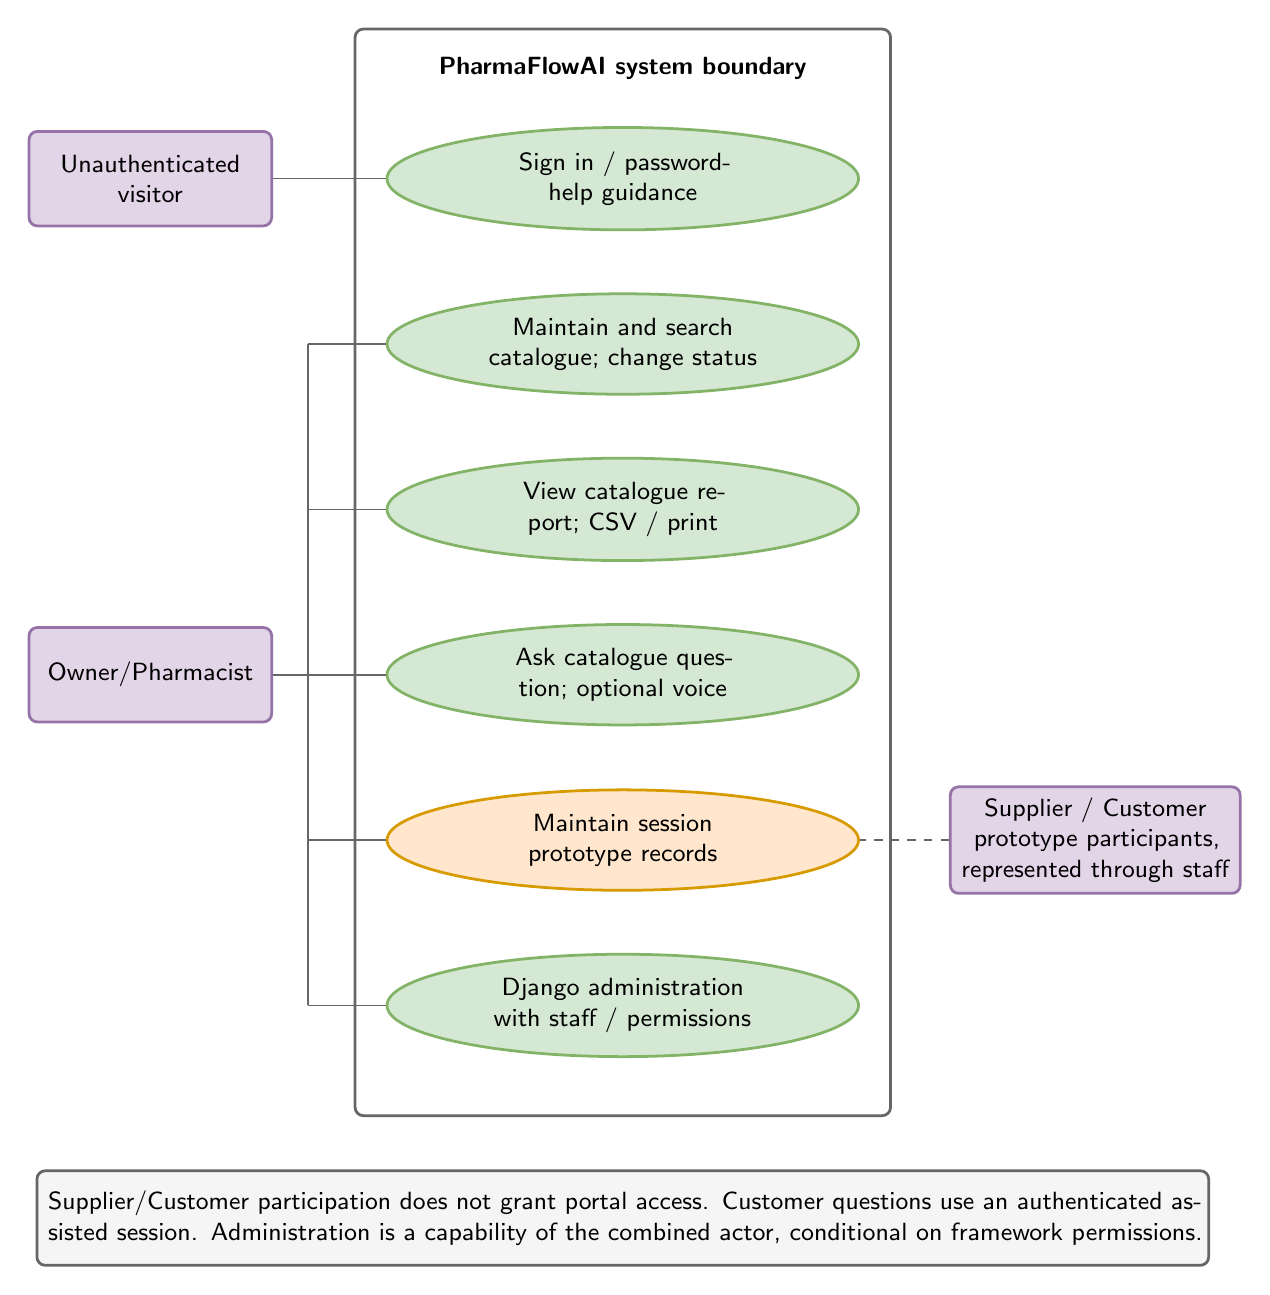
\begin{tikzpicture}
\draw[draw=noteStroke,fill=white,rounded corners=3pt,line width=1pt] (-3.4,1.9) rectangle (3.4,-11.9);
\node[font=\sffamily\small\bfseries] at (0,1.4) {PharmaFlowAI system boundary};
\node[usecase,text width=40mm] (login) at (0,0) {Sign in / password-help guidance};
\node[usecase,text width=40mm] (med) at (0,-2.1) {Maintain and search catalogue; change status};
\node[usecase,text width=40mm] (report) at (0,-4.2) {View catalogue report; CSV / print};
\node[usecase,text width=40mm] (chat) at (0,-6.3) {Ask catalogue question; optional voice};
\node[usecase,text width=40mm,draw=protoStroke,fill=protoFill] (demo) at (0,-8.4) {Maintain session prototype records};
\node[usecase,text width=40mm] (admin) at (0,-10.5) {Django administration with staff / permissions};
\node[actor,text width=28mm] (visitor) at (-6.0,0) {Unauthenticated visitor};
\node[actor,text width=28mm] (owner) at (-6.0,-6.3) {Owner/Pharmacist};
\node[actor,text width=34mm] (part) at (6.0,-8.4) {Supplier / Customer\\prototype participants,\\represented through staff};
\draw[assoc] (visitor.east)--(login.west);
\draw[assoc] (owner.east)--(-4.0,-6.3);
\draw[assoc] (-4.0,-2.1)--(-4.0,-10.5);
\draw[assoc] (-4.0,-2.1)--(med.west);
\draw[assoc] (-4.0,-4.2)--(report.west);
\draw[assoc] (-4.0,-6.3)--(chat.west);
\draw[assoc] (-4.0,-8.4)--(demo.west);
\draw[assoc] (-4.0,-10.5)--(admin.west);
\draw[assoc,dashed] (part.west)--(demo.east);
\node[grey,text width=146mm] at (0,-13.2) {Supplier/Customer participation does not grant portal access. Customer questions use an authenticated assisted session. Administration is a capability of the combined actor, conditional on framework permissions.};
\end{tikzpicture}
}
\caption{Use cases and access boundary. The dashed prototype association denotes business participation, not direct system authorization.}\label{fig:usecase}
\end{figure}

\subsubsection{Use cases and detailed scenarios}
\begin{longtable}{L{26mm}L{121mm}}
\caption{Representative use-case specifications}\\
\toprule Use case & Scenario, alternatives and outcome\\\midrule\endfirsthead
\toprule Use case & Scenario, alternatives and outcome\\\midrule\endhead
\bottomrule\endfoot
UC-01\newline Sign in & \textbf{Actor:} existing active user. \textbf{Precondition:} account has been created. \textbf{Trigger:} submit sign-in. \textbf{Flow:} enter email/username and password, select session preference, validate credentials, establish session, redirect. \textbf{Alternative:} invalid credentials show a generic error; unsafe next destinations are ignored. \textbf{Outcome:} authenticated session or no authenticated state. Maps to FR-AUTH-01--06.\\
UC-02\newline Maintain medicine & \textbf{Actor:} signed-in user. \textbf{Trigger:} Add medicine or Edit. \textbf{Flow:} enter master data, normalize and validate, check uniqueness, save, show details and confirmation. \textbf{Alternative:} missing/duplicate name prevents a successful save. \textbf{Outcome:} persisted valid record. Status changes are separate POST actions. Maps to FR-MED-01--04.\\
UC-03\newline Request report & \textbf{Actor:} signed-in user. \textbf{Trigger:} report link or assistant catalogue-report question. \textbf{Flow:} compute summary, open report, inspect complete register, optionally download CSV or print. \textbf{Alternative:} an empty catalogue shows a zero summary and empty-state message; unauthenticated report access redirects. \textbf{Outcome:} a timestamped report of current catalogue records, not stock or financial balances. Maps to FR-REP-01--04 and FR-VA-03.\\
UC-04\newline Ask by voice & \textbf{Actor:} user at a signed-in session. \textbf{Precondition:} supported browser, secure context and microphone permission. \textbf{Flow:} select language, start microphone, speak a name, review/correct transcript, send, receive catalogue reply, optionally hear it. \textbf{Alternatives:} denial/unsupported voice uses text; medical-pattern query requests pharmacist assistance from the Owner/Pharmacist; unknown medicine uses fallback. \textbf{Outcome:} bounded catalogue assistance; no order or prescription is created. Maps to FR-VA-01--10.\\
UC-05\newline Edit demo record & \textbf{Actor:} signed-in user. \textbf{Trigger:} open a writable module and choose Add/Edit. \textbf{Flow:} supply required fields, save and view changed sample row. \textbf{Alternative:} analytics is read-only; missing fields produce feedback; absent record IDs do not update a different record. \textbf{Outcome:} only the current session payload changes. Maps to FR-DEMO-01--03.\\
\end{longtable}

\subsubsection{Acceptance Criteria for the Current Baseline}
The following acceptance checklist defines completion of the current catalogue-and-assistance scope, not a transactional pharmacy system. Historical automated results are recorded in Section 5.3; remaining manual/environment checks stay To verify.
\begin{enumerate}
\item Valid username/email login creates the selected session policy; invalid/inactive credentials fail; protected pages and chat reject anonymous access.
\item Medicine creation, reading, editing and deactivation/reactivation persist correctly. Name validation and normalized duplicate constraints hold; application deletion is not part of catalogue CRUD here.
\item Search, status/category filters, supported ordering, 20-record pagination and dashboard counts agree with known fixture data.
\item The complete report includes active/inactive records, correct summaries and every CSV row with formula-neutralization. Target-browser print layout is manually checked.
\item English/Hindi catalogue lookup, report intent and medical-pattern fallback behave as specified; reviewed text is sent explicitly and optional voice retains text fallback.
\item Both recorded test commands complete with zero failures. The preserved baseline evidence is 85 Django and 9 JavaScript tests passed on 12 October 2026; this revision does not assert a new run.
\item Prototype modules remain labeled and session-scoped, analytics stays read-only, and no sample figure is represented as a real transaction or inventory balance.
\end{enumerate}
\textbf{Validation acceptance target (To verify).} Across an agreed fixture matrix, reject 100 percent of blank/whitespace-only names and normalized duplicate name/strength/manufacturer combinations; accept distinct strength/manufacturer combinations. Duplicate tests exist in the baseline, but exhaustive coverage and this explicit percentage target have not been measured.

\subsubsection{Known Limitations}
\begin{itemize}
\item No completed billing transactions, payment/tax processing, stock deduction or persistent inventory/batch records.
\item No verified availability, price management, expiry calculation or clinical treatment decision support.
\item No generative AI, persistent conversation history or unrestricted Hindi transliteration; medical routing is pattern-based and non-exhaustive.
\item No supplier/customer portals, enforced permissions derived solely from the stored role label, or email password recovery.
\item No demonstrated production PostgreSQL deployment, load capacity, backup/restore objective or cross-platform certification.
\item Prototype exports lack the catalogue CSV's explicit formula-neutralization. Full reports load the catalogue into memory; speech services and browser print output require environment-specific verification.
\end{itemize}

\subsubsection{Key Features Summary}
\SummaryBox{Implemented: login, medicine catalogue/search, catalogue report/CSV/print and bounded bilingual assistance. Prototype: session operational records and sample analytics. Proposed/To verify: production hardening, persistent operations, scale and environment-specific acceptance.}

\clearpage
\section{Other Nonfunctional Requirements}
\subsection{Performance Requirements}
No load-test report, throughput measurement or production latency objective is present in the project. The implemented list pagination, database indexes and bounded assistant input/result counts are design controls, not proof of a particular capacity. Full-report generation loads the complete catalogue into memory, so its scalability requires measurement.

\begingroup\small\setlength{\tabcolsep}{4pt}
\begin{longtable}{@{}L{25mm}L{88mm}L{16mm}L{22mm}@{}}
\caption{Performance and capacity requirements}\\
\toprule ID & Requirement & Priority & Status\\\midrule\endfirsthead
\toprule ID & Requirement & Priority & Status\\\midrule\endhead
\bottomrule\endfoot
NFR-PER-01 & The medicine list shall paginate at 20 records and use the configured search/sort fields. Verify page boundaries and filter retention in catalogue view tests. & Medium & Implemented\\*
\Criterion{With 21 matching records, page 1 shows 20 and page 2 shows one; search/status/category selections remain in page links.}
NFR-PER-02 & The assistant shall bound message size, candidate processing and displayed results; ordinary matching examines at most 40 selected candidates and displays at most five. Verify boundary inputs and result cardinality. & Medium & Implemented\\*
\Criterion{Submit boundary inputs and a dataset with more than 40 candidates; no successful reply exceeds five displayed medicine results. Candidate-count instrumentation remains To verify.}
NFR-PER-03 & For a separately agreed benchmark of 10 concurrent users and 10,000 catalogue records, target a 95th-percentile response time of at most 2 seconds for list, detail and text-chat requests on a documented reference host. Exclude external speech latency; record hardware, database and test data. This target is not a measured achievement. & Medium & To verify\\*
\Criterion{To verify: proposed k6 HTTP benchmark, 10 concurrent authenticated users, 10,000 seeded records, 2-minute warm-up and 10-minute run; measure endpoint-specific p95, target at most 2 seconds. Reference host CPU/RAM/OS, Python/Django versions, database/version and dataset seed must be recorded and agreed before execution. Exclude browser speech.}
NFR-PER-04 & Benchmark full report and CSV generation at the agreed catalogue size, with an initial target of completion within 10 seconds and no missing records. If memory grows beyond deployment limits, introduce streaming or pagination before increasing capacity claims. & Medium & To verify\\*
\Criterion{To verify: proposed k6 benchmark on the same documented host with 10,000 records; run 30 sequential full-report requests and 30 CSV downloads after warm-up, target p95 at most 10 seconds and 100 percent record completeness. Record peak server memory; acceptable memory ceiling and concurrency remain to be agreed.}
\end{longtable}
\endgroup

\subsection{Security Requirements}
\begingroup\small\setlength{\tabcolsep}{4pt}
\begin{longtable}{@{}L{25mm}L{88mm}L{16mm}L{22mm}@{}}
\caption{Security requirements and limitations}\\
\toprule ID & Requirement & Priority & Status\\\midrule\endfirsthead
\toprule ID & Requirement & Priority & Status\\\midrule\endhead
\bottomrule\endfoot
NFR-SEC-01 & Password verification shall use Django's password hashing/authentication functions, not plaintext comparisons. Stored credentials shall not be displayed in normal application responses. Verify backend usage and generic login failures. & High & Implemented\\*
\Criterion{All invalid-credential test cases leave the client unauthenticated; normal responses contain neither supplied passwords nor stored password hashes.}
NFR-SEC-02 & State-changing forms and chat POST requests shall use CSRF protection. Login-required views shall reject anonymous access. Verify missing-token and unauthenticated requests. & High & Implemented\\*
\Criterion{For every protected page in the route inventory, anonymous GET redirects to login. Anonymous chat POST with a valid CSRF context returns 401; authenticated unsafe requests without a valid token return 403. Target: 100 percent of enumerated cases rejected; complete route-matrix execution is To verify.}
NFR-SEC-03 & Session cookies shall use configured HttpOnly and SameSite policies; unsafe next-page URLs shall not cause external redirects. Verify configuration and redirect tests. & High & Implemented\\*
\Criterion{Every tested external next URL is rejected; a valid local URL is accepted. Inspect HttpOnly/SameSite settings separately from production HTTPS deployment.}
NFR-SEC-04 & Non-debug deployment shall use an explicit secret key, allowed hosts, HTTPS and correctly configured proxy trust. Secure-cookie/HSTS options are present, but a deployment audit is required; default debug settings are not a production configuration. & High & To verify\\*
\Criterion{Conditional on the target environment; Before release, document and pass every applicable deployment-checklist item for secret key, hosts, TLS, cookie flags, HSTS and proxy trust; deployment evidence remains To verify.}
NFR-SEC-05 & Catalogue CSV shall neutralize formula-like text, and chat messages shall be inserted with text-safe DOM operations. Report links shall match the expected local path. Verify malicious cell prefixes and an unexpected external report link. & High & Implemented\\*
\Criterion{Exercise formula-triggering CSV cells, malicious chat text and an external report URL; target zero executable formulas, DOM script insertions or accepted external report links in the agreed fixtures. Full security fixture coverage is To verify.}
NFR-SEC-06 & Define and enforce operation permissions for the combined Owner/Pharmacist actor, covering catalogue mutations and reports with positive and negative tests. Any future supplier/customer portal shall receive only its explicitly authorized access. A role field alone shall not be considered enforcement. & High & Proposed\\*
\Criterion{Proposed: create an operation-by-permission test matrix; require all allowed cases to succeed and all denied cases to fail before calling the policy enforced.}
NFR-SEC-07 & Add login/chat abuse controls and a structured audit trail if production use is approved. Current login/status logging is not a complete, tamper-resistant business audit trail. Specify retention and access rules before implementation. & High & Proposed\\*
\Criterion{Proposed: agree rate limits, audit-event schema, retention and access rules, then test each threshold and logged event. Numeric thresholds are to be agreed.}
\end{longtable}
\endgroup
Customers using a staff-authenticated counter screen share that screen's existing access context. The current application is not a restricted public kiosk. A customer-only permission boundary would require additional design and verification.

\subsection{Software Quality Attributes}
\begingroup\small\setlength{\tabcolsep}{4pt}
\begin{longtable}{@{}L{25mm}L{88mm}L{16mm}L{22mm}@{}}
\caption{Quality attributes and verifiable expectations}\\
\toprule ID & Requirement & Priority & Status\\\midrule\endfirsthead
\toprule ID & Requirement & Priority & Status\\\midrule\endhead
\bottomrule\endfoot
NFR-REL-01 & Ordinary catalogue operations shall retain saved records across sessions and preserve inactive records. Verify create/edit/status persistence. Prototype rows shall remain explicitly session-scoped. & High & Implemented\\*
\Criterion{Create, edit and toggle a record, then read it from another authenticated session; values and identifier remain intact. Confirm that prototype edits do not become shared domain rows.}
NFR-REL-02 & Assistant failures shall restore usable controls and preserve a retryable draft; late cancelled responses shall not reappear after clearing. Verify simulated denial, expiry, cancellation and unavailable-service paths. & High & Implemented\\*
\Criterion{Simulate denial, expiry and cancellation; input controls recover, retryable drafts remain, and zero late replies are appended after clear/close. Network-path coverage is To verify.}
NFR-USA-01 & Forms shall provide labels and validation feedback, lists shall distinguish empty states, and the assistant shall expose status messages and keyboard-operable controls. Verify keyboard paths and accessible names; no formal accessibility conformance claim is made. & Medium & Implemented\\*
\Criterion{Manually traverse sign-in, catalogue form and assistant with the keyboard; each input has an accessible name and every validation error is perceivable. Full manual accessibility results are To verify.}
NFR-USA-02 & Speech shall supplement text. Verify English/Hindi controls on the target browser and device, including unsupported input and unavailable voices. Installed voice quality and recognition accuracy are external dependencies. & Medium & To verify\\*
\Criterion{Conditional on the target environment; Test one supported and one unsupported recognition environment plus denied microphone access; English/Hindi text remains usable in all cases. Record browser/device versions and available voices; live results are To verify.}
NFR-MAI-01 & Accounts, medicines and core functions shall remain separated into Django applications; styling and behaviours shall reside in reusable templates/static assets. Verify module responsibilities and execute relevant regression suites after changes. & Medium & Implemented\\*
\Criterion{Inspect responsibilities of accounts, medicines and core, then run both recorded regression commands; acceptance requires zero failing tests. The historical counts remain 85 Django tests and 9 JavaScript tests.}
NFR-SCA-01 & Validate concurrent catalogue updates and PostgreSQL migration before claiming multi-user production scale. Multi-store tenancy, distributed workers and horizontal scaling are outside the established baseline. & Medium & Proposed\\*
\Criterion{Proposed: agree concurrent-update workloads and a PostgreSQL migration rehearsal; record conflicts, errors and integrity results before asserting capacity.}
NFR-REC-01 & Define and exercise a backup/restore procedure for users, catalogue and configuration before production adoption. Recovery time and permissible data loss must be agreed; neither is established by this repository. & High & Proposed\\*
\Criterion{Proposed, to be agreed: RPO (maximum permissible data loss) and RTO (maximum restoration time). In a restore drill, measure the recovered backup timestamp, elapsed restore time and row-count/integrity checks against the agreed RPO/RTO; no value or successful drill is established.}
NFR-PRI-01 & The application shall not deliberately persist voice audio or chat history, and it shall disclose possible online browser speech processing. Verify page-memory behaviour; provider retention and browser policies require separate review. & High & Implemented\\*
\Criterion{Application behaviour is implemented; external-provider behaviour remains conditional. Clear and reload the page and inspect application storage/network behaviour; no application conversation history is restored and Django receives text, not audio. Browser-provider retention remains To verify.}
\end{longtable}
\endgroup

\subsection{Business Rules}
\begin{enumerate}[label=BR-\arabic*.,leftmargin=19mm]
\item A medicine is catalogue master data, not a batch or a stock balance. A record's existence must not be interpreted as availability for sale.
\item Brand/name, strength and manufacturer together determine case-insensitive catalogue uniqueness after whitespace normalization.
\item Catalogue records default to active; the ordinary list defaults to active records. Inactive records remain accessible through details, status filters and the complete report.
\item The application medicine screens provide deactivation/reactivation rather than deletion. Django administration is a separate privileged interface and is not claimed to prohibit all deletion.
\item Prescription flags reflect data entered into the catalogue. A false flag is reported cautiously and does not certify that a prescription is legally unnecessary.
\item The voice assistant shall not create orders, prescribe medicines, determine treatment suitability or assert unrecorded prices and quantities.
\item Operational sample records shall not be treated as accounting, inventory or customer-history evidence. A session expiration or logout may discard the session context.
\item Only signed-in users can obtain application catalogue reports or use the assistant. Customer-facing wording does not create an anonymous access route.
\item Report totals refer to catalogue records, including inactive records. Dashboard and report category definitions differ where blank categories exist.
\item Data displayed in analytics is demonstrative. No revenue or profit claim may be derived from those predefined values as if calculated from transactions.
\end{enumerate}

\clearpage
\section{Other Requirements}
\subsection{Assumptions and Dependencies}
\begin{itemize}
\item The baseline represents one shared pharmacy catalogue. Multiple tenant isolation is neither modelled nor verified.
\item Accounts are provisioned through authorized administration; public registration is not implemented. Django administration privileges for the combined Owner/Pharmacist actor must be configured independently of the stored role label.
\item Users enter accurate catalogue and prescription-flag data. The system does not validate it against a national drug database or regulatory service.
\item Speech requires a compatible browser, user permission and a suitable environment. Network availability may be required by the browser's provider; text assistance must remain usable without voice.
\item SQLite is the local default. Production database selection, hosting, monitoring and backup arrangements remain decisions to be documented.
\item The supplied reference determines section organization and visual style, not this project's features. Neither reference supplies project features or implementation technologies for \Project.
\item Author names and roll numbers, department, institution and course details were supplied for this revision. Supervisor and submission date remain editable placeholders as requested for this revision; the imported supervisor value is retained only in a source comment.
\end{itemize}

\subsection{Maintenance and Proposed Enhancements}
Maintenance shall keep implementation status visible as the prototype evolves. Database changes require Django migrations and appropriate regression tests. Dependency changes should be tested against authentication, catalogue constraints, reporting and browser behaviour. Secrets and user credentials must not be embedded in documentation or source-controlled configuration.

\begingroup\small\setlength{\tabcolsep}{4pt}
\begin{longtable}{@{}L{25mm}L{88mm}L{16mm}L{22mm}@{}}
\caption{Future work, explicitly outside the implemented baseline}\\
\toprule ID & Requirement & Priority & Status\\\midrule\endfirsthead
\toprule ID & Requirement & Priority & Status\\\midrule\endhead
\bottomrule\endfoot
FUT-01 & Persistent inventory and batches & Medium & Proposed\\*
\Criterion{Required design before acceptance: Batch identifiers, quantities, expiry and prices; validated stock movements and concurrency rules.}
FUT-02 & Transactional billing & Medium & Proposed\\*
\Criterion{Required design before acceptance: Invoice lines, monetary calculation, payments, stock effects, returns and applicable business rules.}
FUT-03 & Supplier/customer domain records & Medium & Proposed\\*
\Criterion{Required design before acceptance: Shared models, relationships, validation, access control and agreed retention.}
FUT-04 & Derived analytics & Medium & Proposed\\*
\Criterion{Required design before acceptance: Defined metrics computed from validated transaction data rather than sample strings.}
FUT-05 & Access control / recovery & Medium & Proposed\\*
\Criterion{Required design before acceptance: Explicit operation permissions and verified email-token password recovery.}
FUT-06 & Expanded assistant & Medium & Proposed\\*
\Criterion{Required design before acceptance: Any generative model, wider language recognition or live-stock tool must have separately specified data access, cost, privacy and accuracy requirements. None is assumed here.}
\end{longtable}\endgroup

\subsubsection{Delivery Phases (Proposed planning sequence)}
No delivery dates or additional completion claims are established. Each phase below is a Proposed plan; phase 1 reviews the already implemented baseline.
\begin{enumerate}
\item \Proposed{} baseline acceptance: validate the implemented catalogue/report/assistant and close outstanding device and permission checks.
\item \Proposed{} persistent inventory: design shared supplier/customer records, batches, quantities, prices and expiry/stock rules (FUT-01, FUT-03).
\item \Proposed{} billing: add validated invoices, payment and stock effects only after inventory integrity is accepted (FUT-02).
\item \Proposed{} analytics: derive agreed measures from validated transactions rather than sample strings (FUT-04).
\item \Proposed{} expanded assistant: specify any additional language, live-stock or model integration, with separate data-access, privacy, accuracy and cost requirements (FUT-06).
\end{enumerate}

\subsection{Verification and Acceptance Mapping}
Verification uses Django tests for server behaviour and Node.js tests that simulate frontend speech events. Simulation avoids collecting microphone audio; it does not establish live recognition quality. The following commands are the repeatable baseline checks:
\begin{quote}\small\ttfamily
py -3.13 manage.py test apps.core apps.accounts apps.medicines --noinput\\
node tests/assistant.test.cjs
\end{quote}

\begin{table}[H]
\centering\small
\caption{Requirement-to-verification mapping}
\begin{tabularx}{\textwidth}{L{39mm}L{49mm}Y}
\toprule Requirement group & Evidence in repository & Additional acceptance work\\\midrule
FR-AUTH; NFR-SEC-01--03 & Account login tests: credentials, expiry, redirects, logout and anonymous access. & Validate browser session-restoration expectations and production HTTPS configuration.\\
FR-MED; FR-DASH & Medicine model/view tests: normalization, uniqueness, filters, pagination, state changes and counts. & Review real-world data entry, keyboard navigation and concurrent updates.\\
FR-REP & Core report tests: counts, full rows, CSV escaping, authentication and empty catalogue. & Visually check pagination and output on target browser print/PDF destinations.\\
FR-DEMO & Core module tests: sample-page rendering and customer add/edit/delete. & Verify remaining demo forms, visible export and intentional session isolation.\\
FR-VA-01--05 & Core assistant tests: live catalogue queries, Hindi alias, medical-pattern routing, report intents and request validation. & Explore ambiguous queries and unsupported aliases; do not infer conversational intelligence.\\
FR-VA-06--10 & Nine JavaScript tests: transcript review, fallback, denied access, close/clear cancellation, read-aloud, expiry and report-link checks. & Test microphone capture and audible English/Hindi output on the actual customer device.\\
Proposed NFRs & No benchmark/deployment proof established. & Execute the agreed load, permissions, recovery and platform validation plans before claiming compliance.\\
\bottomrule
\end{tabularx}
\end{table}

\subsubsection{Detailed requirement traceability}
Each TC identifier below is an acceptance scenario, not a newly executed test or a one-to-one claim about a source test function. ``Passed in baseline'' is used only for scenarios supported by the original document's stated automated evidence. A requirement may be implemented while an additional acceptance scenario is still To verify. Django evidence refers to S09; simulated Node evidence refers to S10. Manual evidence means a planned check, not a completed observation.
\begingroup\scriptsize\setlength{\tabcolsep}{2.5pt}
\begin{longtable}{@{}L{9mm}L{26mm}L{41mm}L{29mm}L{20mm}L{21mm}@{}}
\caption{Traceability: authentication, catalogue, reports and prototypes}\label{tab:trace-core}\\
\toprule Test ID & Scenario & Expected result & Requirement IDs & Evidence & Status\\\midrule\endfirsthead
\toprule Test ID & Scenario & Expected result & Requirement IDs & Evidence & Status\\\midrule\endhead
\bottomrule\endfoot
TC-01 & Login using supported credentials & Valid username/email establishes an authenticated session. & FR-AUTH-01 & Django test & Passed in baseline\\
TC-02 & Invalid credentials & Generic error; no authenticated session. & FR-AUTH-02; NFR-SEC-01 & Django test & Passed in baseline\\
TC-03 & Inactive account & Authentication denied. & FR-AUTH-02 & Django test (planned detail) & To verify\\
TC-04 & Remember me policies & Configured age versus browser-close session semantics. & FR-AUTH-03 & Django test & Passed in baseline\\
TC-05 & Local / external next URL & Local destination accepted; external redirect rejected. & FR-AUTH-06; NFR-SEC-03 & Django test & Passed in baseline\\
TC-06 & Logout and protected access & Logout ends session; later protected requests require login. & FR-AUTH-04--05 & Django test & Passed in baseline\\
TC-07 & Create, read, edit medicine & Valid values persist and details reflect the saved record. & FR-MED-01,03; NFR-REL-01 & Django test (planned detail) & To verify\\
TC-08 & Required medicine name & Blank and whitespace-only names rejected in every agreed fixture. & FR-MED-01 & Django test (planned detail) & To verify\\
TC-09 & Normalization and duplicates & Whitespace normalized; equivalent name/strength/manufacturer rejected. & FR-MED-02 & Django test & Passed in baseline\\
TC-10 & Medicine status changes & Status toggles; record retained. & FR-MED-04 & Django test & Passed in baseline\\
TC-11 & GET status / missing record & GET does not mutate; nonexistent detail/edit ID returns 404. & FR-MED-03--04 & Django test (planned detail) & To verify\\
TC-12 & Search and filters & Matching fields and status/category select expected rows. & FR-MED-05 & Django test & Passed in baseline\\
TC-13 & Pagination & 20-record page boundary and filter retention. & FR-MED-06; NFR-PER-01 & Django test & Passed in baseline\\
TC-14 & Empty and no-match list & Initial creation prompt differs from a filtered no-match message. & FR-MED-07 & Manual & To verify\\
TC-15 & Dashboard counts & Counts agree with Medicine records; sample values remain labeled. & FR-DASH-01--02 & Django test (counts); Manual (labels) & To verify\\
TC-16 & Full / empty catalogue report & All rows and expected counts; empty dataset handled. & FR-REP-01--02 & Django test & Passed in baseline\\
TC-17 & Authenticated CSV and escaping & Full CSV rows, proper field escaping; anonymous report access denied. & FR-REP-03; FR-AUTH-04 & Django test & Passed in baseline\\
TC-18 & CSV formula prefixes & Formula-like text is neutralized for every agreed malicious fixture. & FR-REP-03; NFR-SEC-05 & Django test (planned detail) & To verify\\
TC-19 & Print / save PDF & Navigation hidden; readable landscape A4 output on target browser. & FR-REP-04 & Manual & To verify\\
TC-20 & Prototype rendering and customer mutations & Sample pages render; customer add/edit/delete changes session payload. & FR-DEMO-01--02 & Django test & Passed in baseline\\
TC-21 & Other demos and session isolation & Remaining forms/export work; another session does not share mutations. & FR-DEMO-01--03 & Manual & To verify\\
TC-22 & Read-only analytics & No add/edit controls or successful mutation; figures remain samples. & FR-DEMO-03 & Manual & To verify\\
\end{longtable}\endgroup

\begingroup\scriptsize\setlength{\tabcolsep}{2.5pt}
\begin{longtable}{@{}L{9mm}L{26mm}L{41mm}L{29mm}L{20mm}L{21mm}@{}}
\caption{Traceability: chatbot, voice and outstanding nonfunctional checks}\label{tab:trace-assistant}\\
\toprule Test ID & Scenario & Expected result & Requirement IDs & Evidence & Status\\\midrule\endfirsthead
\toprule Test ID & Scenario & Expected result & Requirement IDs & Evidence & Status\\\midrule\endhead
\bottomrule\endfoot
TC-23 & English catalogue lookup & Current catalogue data used for a recognized medicine query. & FR-VA-01--02 & Django test & Passed in baseline\\
TC-24 & Supported Hindi alias & Supported Hindi query maps to the expected catalogue search. & FR-VA-05 & Django test & Passed in baseline\\
TC-25 & Medical-pattern question & Bounded routing to pharmacist assistance; no treatment generated. & FR-VA-04 & Django test & Passed in baseline\\
TC-26 & Catalogue report intent & Counts and local report link returned. & FR-VA-03 & Django test & Passed in baseline\\
TC-27 & Request validation & Invalid request schema rejected rather than producing a successful reply. & FR-VA-01 & Django test & Passed in baseline\\
TC-28 & Exact validation boundaries & Empty/501-character text, invalid language, malformed JSON and non-string message return 400. & FR-VA-01; NFR-PER-02 & Django test (planned detail) & To verify\\
TC-29 & Anonymous chat with CSRF context & 401 when not rejected earlier by CSRF. & FR-AUTH-04; NFR-SEC-02 & Django test (planned detail) & To verify\\
TC-30 & Missing CSRF token & Authenticated unsafe chat request rejected with 403. & NFR-SEC-02 & Django test (planned detail) & To verify\\
TC-31 & Oversized chat body & Body above 8,192 bytes rejected with 413 when handled by the view. & FR-VA-01; NFR-PER-02 & Django test (planned detail) & To verify\\
TC-32 & Transcript review & Recognition fills editable draft; no automatic chat request. & FR-VA-06 & Node test & Passed in baseline\\
TC-33 & Unsupported / denied recognition & Listening releases and typing remains available. & FR-VA-08 & Node test & Passed in baseline\\
TC-34 & Opt-in read-aloud & Playback follows opt-in controls and is cancellable. & FR-VA-07 & Node test & Passed in baseline\\
TC-35 & Expired session & Failure handled with usable controls. & FR-VA-09; NFR-REL-02 & Node test & Passed in baseline\\
TC-36 & Clear / close during request & Cancelled/late responses do not repopulate cleared chat. & FR-VA-09--10 & Node test & Passed in baseline\\
TC-37 & Client timeout & Pending request aborted after configured 15 seconds; draft remains retryable. & FR-VA-09; NFR-REL-02 & Node test (planned detail) & To verify\\
TC-38 & Untrusted report link & Unexpected external link is not accepted. & FR-VA-03; NFR-SEC-05 & Node test & Passed in baseline\\
TC-39 & Live English/Hindi speech & Actual device captures speech and plays selected-language output when supported. & FR-VA-05--08; NFR-USA-02 & Manual & To verify\\
TC-40 & Page-memory history cap & No restored chat after reload; at most 40 message elements retained. & FR-VA-10; NFR-PRI-01 & Manual & To verify\\
TC-41 & Performance and report completeness & Proposed p95 targets and record completeness met under the specified benchmark. & NFR-PER-03--04 & Manual (k6 plan) & To verify\\
TC-42 & Deployment, permissions and recovery & Agreed deployment checklist, operation matrix and backup/restore drill pass. & NFR-SEC-04,06--07; NFR-REC-01 & Manual & To verify\\
\end{longtable}\endgroup

\textbf{Baseline verification note.} Both suites were re-executed on \BaselineDate: all 85 Django tests and all nine JavaScript tests passed. Django's system check reported no issues. The launcher also emitted a Python-location warning, but the test run completed successfully. Automated test results are bounded evidence and do not establish production readiness.

\subsection{Reference Alignment and Document Control}
The original five numbered chapters and their existing subsections are retained. Definitions and references are consolidated into Sections 1.4 and 1.5, with pointers preserved in Sections 5.5 and 5.6. New third-level subsections add permissions, constraints, diagrams and acceptance planning without removing existing requirements.

The original S01 reference supplied the chapter hierarchy and academic presentation. The additional R04 reference supplies only visual and structural ideas: pastel diagram palettes, layered architecture, explicit diagram boundaries and document-control information. All actors, data and requirements remain PharmaFlowAI-specific. DFDs represent logical information flows; the class/ER view represents the actual data model. Use-case and state diagrams clarify existing interactions rather than establish new features.

Serif body text, sans-serif numbered headings, A4 pages, contents, lists of figures/tables, numbered captions and page numbers are retained. Page count follows the content rather than a reference document's length. Version remains 1.0 and the implementation baseline remains 12 October 2026. This editorial revision does not claim new test results.

\subsection{Source References}
The complete source list S01--S10 is retained in Section~\ref{sec:references}. S01 records the original structural reference; R04 records the additional visual reference used for this revision.

\subsection{Terminology}
The original terminology is merged into the two-column definitions table in Section~\ref{sec:terms}.
\end{document}